\documentclass[10pt]{article}
\usepackage[margin=0.65in]{geometry}
\usepackage{amsmath,amssymb,amsthm,mathtools,enumitem,microtype,booktabs}
\usepackage{graphicx}
\usepackage[compact]{titlesec}
\usepackage[hidelinks]{hyperref}
\usepackage{cleveref}
\titlespacing*{\section}{0pt}{3pt}{1pt}
\titlespacing*{\subsection}{0pt}{2pt}{1pt}
\setlist{nosep,leftmargin=*}
\setlength{\parskip}{2pt}\setlength{\parindent}{0pt}
\setlength{\tabcolsep}{4pt}

% ---------- theorem environments (shared counter) ----------
\theoremstyle{plain}
\newtheorem{theorem}{Theorem}
\newtheorem{lemma}[theorem]{Lemma}
\newtheorem{proposition}[theorem]{Proposition}
\newtheorem{corollary}[theorem]{Corollary}
\theoremstyle{definition}
\newtheorem{definition}[theorem]{Definition}
\newtheorem{assumption}{Assumption}
\renewcommand{\theassumption}{A\arabic{assumption}}
\theoremstyle{remark}
\newtheorem{remark}[theorem]{Remark}
\crefname{assumption}{assumption}{assumptions}
\crefname{proposition}{Proposition}{Propositions}

% ---------- macros ----------
\newcommand{\R}{\mathbb{R}}
\newcommand{\E}{\mathbb{E}}
\newcommand{\Hbar}{\bar H}
\newcommand{\epss}{\varepsilon_s}
\newcommand{\epsv}{\varepsilon_v}
\newcommand{\etaNL}{\eta_{\mathrm{NL}}}
\newcommand{\Ahat}{\hat A}
\newcommand{\Qhat}{\hat Q}
\newcommand{\Qstar}{Q^\star}
\newcommand{\Vstar}{V^\star}
\newcommand{\Dbar}{\bar\Delta}
\DeclareMathOperator{\val}{val}
\DeclareMathOperator{\expl}{expl}
\DeclareMathOperator{\TV}{TV}
\DeclareMathOperator{\Reg}{Reg}
\DeclareMathOperator{\range}{range}
\DeclareMathOperator{\lgs}{lgs}
\DeclareMathOperator{\gain}{gain}
\DeclareMathOperator*{\argmin}{arg\,min}
\DeclareMathOperator*{\argmax}{arg\,max}

\title{\vspace{-2.4em}\textbf{Per-Turn Equilibrium Play in Pok\'emon Random Battles:\\Error Budgets, Regret over Experts, and Measured Exploitability}\vspace{-0.8em}}
\author{CS535 Final Report \quad [Name 1], [Name 2]}
\date{\vspace{-1.6em}}

\begin{document}
\maketitle

\begin{abstract}
\noindent
We model Gen~9 Random Battles as a finite-horizon, two-player, zero-sum stochastic game with simultaneous moves, chance and hidden information, and study an agent that, every turn, builds a stage matrix (one simulated turn plus a heuristic leaf value) and solves it with Regret Matching$^+$ (RM$^+$). On the theory side we prove that exploitability is at most $\Hbar(\epss+2\epsv+\text{sampling})$, where $\Hbar$ is the expected game length against a best response (not the typical length), and that the leaf term $\epsv$ does not shrink with compute. Under hidden information two further terms appear, a non-locality gap and a belief error, and both are necessary. On top of the per-turn agent we place Hedge over an MCTS expert and an equilibrium expert, prove safety relative to the surrogate matrix and an across-game bound for the shipped anytime update, and document a linear-regret bug in our first anytime implementation. Empirically, time-matched foul-play-style MCTS beats equilibrium play (0.760 [0.677, 0.843] vs.\ equilibrium sampled), while equilibrium sampling is less exploitable by a one-turn local best response. A depth-2 white-box exploiter confirms it at 100 pairs (0.873 vs.\ 0.713 for top move vs.\ sampled). Carrying Hedge weights across games makes the learner significantly harder to exploit (paired difference $+0.146$ [$+0.039$, $+0.253$]). Exact endgame solutions point to the leaf value as the bottleneck. We report confidence intervals throughout and mark preliminary results.
\end{abstract}

% =====================================================================
\section{Introduction}
\label{sec:intro}
A Pok\'emon battle is a winner-take-all game played under uncertainty. Both players choose at the same time, damage rolls, accuracy and critical hits are random, and in Random Battles each side's sets (moves, item, ability, Tera type) are drawn from a known generator and stay hidden until revealed. Our proposal planned a Bayesian memory over the opponent's set and style, a no-regret per-turn solver, and an evaluation ``status card'' (worst case, predictable opponents, equals). This report covers the parts we carried out and adds a theory of the per-turn agent that the proposal only listed as a goal (the ``error budget'').

\textbf{The agent.} Each turn the agent enumerates both sides' legal actions, simulates one turn exactly over chance outcomes in the Rust engine poke-engine, scores each child position with a heuristic leaf, and solves the resulting stage matrix with RM$^+$. Under hidden information it samples $K$ opponent worlds and solves one agent-form game over them. Across turns and games, a Hedge learner mixes this equilibrium expert with an MCTS expert.

\textbf{What we contribute.}
\begin{enumerate}[label=(\arabic*)]
\item \emph{An error budget for per-turn solving} (\cref{sec:theory}), our main step beyond the course's no-regret analysis of one repeated matrix game (\cref{sec:prelim}): we compose per-turn $\epss$-equilibria of estimated stage matrices through a finite-horizon stochastic game with leaf error, giving $\expl\le\Hbar(\epss+2\epsv+\text{sampling})$, with $\Hbar$ the best-response length and a counterexample showing typical length does not suffice; explicit RM$^+$ and sampling rates; and a five-term hidden-information version whose two extra terms are both necessary. The core steps are Lean-checked.
\item \emph{A regret layer with stated guarantees} (\cref{sec:regret}), framed as the experts problem against an adaptive opponent: safety of Hedge over experts relative to the surrogate matrix, an across-game bound for the shipped anytime FTRL, a closed-form linear-regret rate for the incremental anytime update we first shipped, and a weight-dynamics identity that explains why carried weights resist an exploiter.
\item \emph{Exploitability measurement with explicit lower and upper sides} (\cref{sec:measure}): any fixed exploiter gives a valid lower bound, with a selection correction, and we show what the ``exploitation gain'' does and does not certify. A 100-pair white-box run certifies positive lower bounds for both equilibrium targets (0.250 top move, 0.090 sampled).
\item \emph{Leaf diagnostics} (\cref{sec:leaf}): affine invariance, why a single mis-scored terminal forces the best affine calibration to be constant, and a minimal non-termination example.
\item \emph{Experiments} (\cref{sec:exp}), with 95\% CIs, including exact-endgame measurements of true exploitability.
\end{enumerate}
We make no ladder or Showdown claims: we never played on the Showdown ladder, and we make no comparison with Jaxcalibur or any other ladder bot. The agent-form formulation itself comes from PokaiTrainer~\cite{Yu26}; we evaluate it, we did not invent it.

% =====================================================================
\section{Related work}
\label{sec:related}
\textbf{Pok\'emon agents.} Foul Play~\cite{foulplay} samples opponent sets from count-weighted data and runs decoupled-UCT MCTS per sample in poke-engine, then sums visit fractions and samples among moves within 75\% of the top fraction. It won the PokeAgent Gen~9 OU final~\cite{pokeagent}. Jaxcalibur (self-reported, closed source; a Smogon post and a write-up only) combines self-play PPO with a regret-flavoured pUCT over 32 sampled worlds~\cite{jaxcalibur}.
Chronoquazicalar (a hobby repository) solves a root regret-matching matrix per sampled world and averages the results~\cite{chrono}.
PokaiTrainer~\cite{Yu26} solves every VGC decision as a Bayesian matrix game with CFR, under open team sheets. Other lines use LLMs (Pok\'eChamp~\cite{Kar25}, PokeLLMon~\cite{hu2024pokellmon}), offline RL on replays (Metamon~\cite{grigsby2025metamon}), or MCTS with PPO (Wang~\cite{wang2024randbats}). ISMCTS was evaluated for Pok\'emon in~\cite{Iha18}. Per-turn matrix solving plus world sampling is therefore not new as a system. Our contribution is the analysis and the measurement.

\textbf{Game theory.} Stage-wise backward induction for stochastic games goes back to Shapley~\cite{Shapley53}. Strategy fusion and non-locality in determinized search are due to Frank and Basin~\cite{Fra98} and Long et al.~\cite{Lon10}. Safe re-solving with range-dependent leaves (CFR-D~\cite{CFRD}, DeepStack~\cite{Mor17}, safe subgame solving~\cite{Bro17}, depth-limited solving~\cite{Bro18}, ReBeL~\cite{Bro20}, value functions over public states~\cite{Kov23}) is exactly what removes our non-locality term. RM$^+$ comes from~\cite{Tam14,Tammelin15}, and its alternating-update analysis from Burch, Moravčík and Schmid~\cite{BMS19}. No external regret goes back to Hannan~\cite{Hannan57} and weighted majority to Littlestone and Warmuth~\cite{LW94}; Hedge, fixed share and anytime tuning come from~\cite{FS97,HW98,CBL06}, policy regret from~\cite{Aro12b}, and safe exploitation from~\cite{Gan15,Joh09}. Simultaneous-move search and pruning are covered by~\cite{Saf12,Bos16,Lis13}, and approximate exploitability via learned best responses by~\cite{Tim20}. Non-termination in undiscounted games goes back to Everett's recursive games~\cite{Everett57} and the Dubins--Savage thrifty/equalizing characterisation~\cite{DS65,MS96}.

% =====================================================================
\section{Preliminaries: no-regret learning and games}
\label{sec:prelim}
This section collects the background from the course's lecture notes~\cite{CS535L6} that the rest of the report builds on, in their notation. Our agent uses one principle, no-regret learning, at three levels: inside a turn (RM$^+$ self-play on the stage matrix, \cref{sec:setting,sec:theory}), across turns and games (Hedge over experts, \cref{sec:regret}), and, as a lens, inside MCTS (\cref{sec:links}).

\textbf{The experts problem.} There are $n$ experts and a horizon of $T$ rounds. In round $t$ Nature fixes a loss $l^t_i\in[0,1]$ for every expert $i$. Without seeing these losses, the algorithm chooses a distribution $p^t$ over the experts and follows an expert drawn from it; Nature then reveals all the losses, and the algorithm incurs the loss of the expert it followed. \emph{Adversary model:} the losses may depend on everything that happened earlier, and Nature may know the algorithm and hence $p^t$, but not the current random draw from $p^t$.

\textbf{External regret.} The regret is the algorithm's expected total loss minus the total loss of the best fixed expert in hindsight,
\[
\Reg_T=\sum_{t\le T}p^t\cdot l^t-\min_i\sum_{t\le T}l^t_i ,
\]
and an algorithm is \emph{no-regret} if $\Reg_T=o(T)$, so that its average regret per round vanishes. This comparison with the best fixed action is Hannan's~\cite{Hannan57} and is called external regret. \emph{Deterministic algorithms fail.} Follow-the-leader (FTL) picks the expert with the smallest cumulative loss. With two experts, Nature can give loss 1 to whichever expert FTL is about to follow and 0 to the other; after the first round the cumulative losses always differ by $\frac12$, FTL switches to the wrong expert every round, and its regret is at least $T/2-1$. The same construction applies to any deterministic map from past losses to an expert, since Nature can compute its next choice. Beating an adversary therefore requires a randomised algorithm, whose current draw Nature cannot see.

\textbf{Multiplicative weights.} The multiplicative weights update (MWU; randomised weighted majority~\cite{LW94}, Hedge~\cite{FS97}) fixes $\eta\in(0,\frac12]$, starts from $w^1_i=1$, plays $p^t_i=w^t_i/\sum_jw^t_j$, and updates $w^{t+1}_i=w^t_i(1-\eta l^t_i)$. The potential $W^t=\sum_iw^t_i$ satisfies $W^{T+1}=n\prod_t(1-\eta L^t_{\rm MWU})$, where $L^t_{\rm MWU}=p^t\cdot l^t$, and $W^{T+1}\ge(1-\eta)^{L^*}$ with $L^*$ the best expert's total loss. Taking logarithms and using $\ln(1-x)\le-x$ and $-\ln(1-\eta)\le\eta+\eta^2$,
\[
L_{\rm MWU}\le(1+\eta)L^*+\frac{\ln n}{\eta},
\]
so for $T\ge4\ln n$ and $\eta=\sqrt{\ln n/T}$ the regret is at most $2\sqrt{T\ln n}$.

\textbf{No-regret self-play in a zero-sum matrix game.} Let $A\in[0,1]^{n\times m}$ be the payoff to the row player (Row, maximiser) and the loss of the column player (Column), with $v_R=\max_x\min_yx^\top Ay$ and $v_C=\min_y\max_xx^\top Ay$; weak duality gives $v_R\le v_C$. Both players run a no-regret algorithm in the full-information model: at each round Row feeds its algorithm the loss $1-e_i^\top Ay^t$ for each row $i$, and Column the loss $(x^t)^\top Ae_j$ for each column $j$. Let $\bar x=\frac1T\sum_tx^t$ and $\bar y=\frac1T\sum_ty^t$ be the average strategies, $\bar g=\frac1T\sum_t(x^t)^\top Ay^t$ Row's average payoff, and $\epsilon_R,\epsilon_C$ the two players' average regrets.
\begin{proposition}[no-regret self-play gives an approximate minimax equilibrium~\cite{FS97,CS535L6}]\label{prop:selfplay}
$v_C-\epsilon_R\le\bar g\le v_R+\epsilon_C$, and
\[
\max_xx^\top A\bar y-\min_y\bar x^\top Ay\le\epsilon_R+\epsilon_C .
\]
Hence $(\bar x,\bar y)$ is an $(\epsilon_R+\epsilon_C)$-approximate minimax equilibrium, and $\min_y\bar x^\top Ay\ge\val(A)-\epsilon_R-\epsilon_C$.
\end{proposition}
\begin{proof}[Proof idea]
Row's no-regret guarantee and linearity give $\bar g\ge\max_i\frac1T\sum_te_i^\top Ay^t-\epsilon_R=\max_xx^\top A\bar y-\epsilon_R\ge v_C-\epsilon_R$, because $\bar y$ is one strategy Column could use. Symmetrically, $\bar g\le\min_y\bar x^\top Ay+\epsilon_C\le v_R+\epsilon_C$. Rearranging gives the gap bound; as $\epsilon_R,\epsilon_C\to0$ it proves the minimax theorem $v_R=v_C$.
\end{proof}
Three remarks set up how we use it. (i) The proof uses only the two regret inequalities and linearity, so it holds for any pair of no-regret algorithms, not only MWU, and for weighted averages $\bar x=\sum_t\alpha_tx^t/\sum_t\alpha_t$ when $\epsilon_R,\epsilon_C$ are the correspondingly weighted average regrets. (ii) For a matrix with payoff range $\Delta$ instead of $[0,1]$ the regrets, and hence the gap, scale by $\Delta$. (iii) In general-sum games, the time-average joint play of no-regret learners is an approximate coarse correlated equilibrium (CCE). Our game is two-player zero-sum, where the marginals of a CCE are minimax strategies, so CCE adds nothing here and we do not use it.

\textbf{Exploit, but retreat to safety.} The lectures motivate the experts problem with a rock-paper-scissors ``hustler'': the minimax strategy guarantees breaking even, but against a hustler with a tell it leaves money on the table, and we want an algorithm that exploits the flaw yet retreats to the safe equilibrium when the hustler plays perfectly. This is the design goal of our Hedge layer (\cref{sec:regret}) and of safe opponent exploitation~\cite{Gan15}. Two further points from the lectures recur in our results. Against a stationary Nature, randomising does not pay: if a screen shows green 70\% of the time, matching the frequencies succeeds 58\% of the time while always guessing green succeeds 70\%. And no-regret learning, though a poor model of human play, is a natural benchmark for algorithmic agents such as ours.

\textbf{What the lectures do not cover.} \Cref{prop:selfplay} concerns repeated play of \emph{one} matrix game whose payoffs are known. In a battle every turn has a new stage matrix, that matrix is only an estimate whose cells use a heuristic leaf, and the turns are linked through a finite-horizon stochastic game whose length the opponent can influence. Composing per-turn $\epss$-equilibria of estimated stage matrices through this game, with the leaf error charged explicitly, is our main step beyond the lectures (\cref{sec:theory}).

% =====================================================================
\section{Setting and agent}
\label{sec:setting}
\textbf{Game.} We use a finite-horizon, two-player, zero-sum stochastic game with finite states, horizon $H$, terminal payoffs in $[-1,1]$ (win $+1$, draw or 300-turn cap $0$, loss $-1$), simultaneous actions $a\in A(s)$, $\beta\in B(s)$ and chance transitions $P(\cdot\mid s,a,\beta)$. The true stage matrix is $\Qstar_t(s)(a,\beta)=\sum_{s'}P(s'\mid s,a,\beta)\Vstar_{t+1}(s')$, and $\Vstar_t(s)=\val\Qstar_t(s)$, where $\val(A)=\max_x\min_y x^\top Ay$. The agent is the row player (maximizer). Exploitability is $\expl(\pi)=\Vstar_0(s_0)-\inf_\sigma W^{\pi,\sigma}_0(s_0)$, where the opponent $\sigma$ may condition on the whole history. In payoff units every stage matrix has range $\Delta\le2$. Score units are $s=(u+1)/2$, so exploitability in score units is half the payoff-unit value.

\textbf{Per-turn agent.} At live $(t,s)$ the agent builds $\Qhat_t(s)$ (\texttt{nash.full\_matrix}): an unpruned depth-2 expectiminimax matrix whose cells average the leaf over all chance outcomes. The leaf is the midpoint of the two sides' maximin values from the engine's depth-1 search, in heuristic engine units. It then runs $T$ iterations of RM$^+$ with alternating updates and linear averaging (\texttt{nash.rm\_plus}); this is the no-regret self-play of \cref{prop:selfplay} on $\Qhat_t(s)$, with full-information feedback. It departs from the lectures' dynamics in two ways: the updates alternate (Column's iterate responds to Row's new iterate), and the average is weighted by $t$ rather than uniform. \Cref{prop:selfplay} goes through with $t$-weighted regrets (remark (i)), and alternation adds a cross term that is $\le0$ for RM$^+$ (\cref{prop:rm}). It plays the averaged strategy (``equilibrium, sampled''), its most probable action (``equilibrium, top move''), or the pure maximin row (``safest move''). \Cref{tab:notation} lists the notation.

\textbf{Hidden information.} Each side sees its own team and what the opponent has revealed. The belief is the exact posterior over each revealed Pok\'emon's sets given revealed moves and Tera type (hard evidence only). The agent-form agent samples $K=4$ worlds and solves $\max_x\sum_k b_k\min_j(M_k^\top x)_j$ as one LP, with the opponent best-responding in each world. The PIMC blend averages the per-world equilibria instead.

\textbf{Experts learner.} This is the experts problem of \cref{sec:prelim} with the real opponent as Nature. The learner keeps weights $w_t$ over $k$ experts with stage strategies $q_{e,t}$ and plays $p_t=\sum_e w_{t,e}q_{e,t}$. After seeing the opponent's move $b_t$ it rewards every expert counterfactually,
$r_{t,e}=\mathrm{clip}\big((q_{e,t}\cdot\Ahat_t[:,b_t]-\min\Ahat_t)/\Dbar,0,1\big)$ with $\Dbar=400$ engine units. The shipped update is anytime FTRL, $\log w_t=\eta_{t-1}L_{t-1}$ with $L_t=\sum_{s\le t}r_s$ and $\eta_t=\sqrt{8\ln k/t}$. \texttt{Hedge2} uses $k=2$ experts: $F$ (foul-play-style MCTS) and $N$ (RM$^+$ equilibrium, sampled).

\begin{table}[t]
\centering\small
\caption{Notation. Each symbol keeps one meaning throughout.}
\label{tab:notation}
\begin{tabular}{@{}ll@{\qquad}ll@{}}
\toprule
$n,m$ & legal actions of agent / opponent in a turn ($\le13$) & $k$ & number of experts \\
$\Delta$ & payoff range of a stage matrix ($\le2$) & $w_t,\ p_t$ & expert weights; played mixture \\
$T$ & RM$^+$ iterations per turn & $r_t,\ L_t$ & expert rewards in $[0,1]^k$; cumulative rewards \\
$K$ & sampled opponent worlds & $\eta_t,\ \beta_t$ & $\sqrt{8\ln k/t}$; step used at turn $t$ ($\beta_t=\eta_{t-1}$) \\
$\epss$ & solver gap in the estimated stage matrix & $G_t,\ d_t$ & $L_{t,N}-L_{t,F}$; $r_{t,N}-r_{t,F}$ \\
$\epsv$ & leaf error $\lVert\Qhat_t(s)-\Qstar_t(s)\rVert_\infty$ & $\Dbar$ & fixed reward normaliser (400 engine units) \\
$\Hbar$ & expected length against a best response & $S,\ N$ & non-forced learner turns; games in a match \\
$\etaNL$ & non-locality gap (\cref{sec:general}) & $v^\star$ & game value in score units ($=1/2$) \\
$\TV$ & total variation, true posterior vs.\ our belief & $\nu,\ m_X$ & evaluation pairs; number of exploiters tried \\
\bottomrule
\end{tabular}
\vspace{-0.6em}
\end{table}

% =====================================================================
\section{Theory of the per-turn agent}
\label{sec:theory}
\Cref{prop:selfplay} bounds the quality of one stage solution in one known matrix. This section composes those per-turn solutions, each an $\epss$-equilibrium of an \emph{estimated} matrix $\Qhat_t(s)$, through the finite-horizon stochastic game, which the lectures do not cover. Assumptions for the main bound:
\begin{assumption}[non-revealing opponent]\label{asm:nonrev} The opponent's moves do not depend on its hidden sets, so behavioural evidence does not move our belief away from the truth. This holds trivially under full information.\end{assumption}
\begin{assumption}[world-only leaves]\label{asm:world} The value after the lookahead depends on the true position, not on what each side believes. Concealment then has no value.\end{assumption}
\begin{assumption}[exact prior]\label{asm:prior} Opponent sets are drawn from the Random Battle generator, which we sample from directly.\end{assumption}

\begin{lemma}[one turn]\label{lem:one}
Let $\lVert A-B\rVert_\infty\le\varepsilon$ and let $x$ be $\epss$-optimal in $B$. Then $\min_y x^\top Ay\ge\val(A)-\epss-2\varepsilon$. The factor $2$ is tight.
\end{lemma}
\begin{proof}[Proof sketch]
$|x^\top(A-B)y|\le\varepsilon$ for all mixed $x,y$, hence $|\val A-\val B|\le\varepsilon$. Apply the first bound once more to $x$. Tightness: $A=(0,-2\varepsilon)^\top$, $B=(-\varepsilon,-\varepsilon)^\top$, $x=e_2$. Lean: \texttt{lemma1\_one\_step}, \texttt{lemma1\_mixed}, with the tightness instance.
\end{proof}

\begin{theorem}[whole game, full information]\label{thm:full}
Let the agent be Markov, with $\lVert\Qhat_t(s)-\Qstar_t(s)\rVert_\infty\le\epsv$ and $\epss$-optimal stage play, and put $\delta=\epss+2\epsv$. For every history-dependent opponent $\sigma$,
$W^{\pi,\sigma}_0(s_0)\ge\Vstar_0(s_0)-\E_{\pi,\sigma}\big[\sum_{t<\tau}\delta(t,s_t)\big]$. Hence, for a best response $\sigma^\star$ with $\Hbar=\E_{\pi,\sigma^\star}[\tau]$,
\begin{equation}\label{eq:full}
\expl(\pi)\;\le\;\E_{\pi,\sigma^\star}\Big[\sum_{t<\tau}\delta(t,s_t)\Big]\;\le\;\Hbar\,(\epss+2\epsv)\;\le\;H(\epss+2\epsv).
\end{equation}
\end{theorem}
\begin{proof}[Proof sketch]
Backward induction over histories: $W_t(h)\ge\Vstar_t(s_t)-D_t(h)$, where $D_t$ is the conditional sum of remaining budgets. The step uses \cref{lem:one} at the opponent's actual stage mixture. The induction is Lean-checked in abstract form (\texttt{theoremA\_abstract}). The link from the game model to the abstract kernel was checked by reading (\cref{app:status}).
\end{proof}

\begin{remark}[$\Hbar$ cannot be the typical length]\label{rem:hbar}
Take states $s_c$ and terminals $z_c$ with $u(z_c)=-c\delta$. The agent picks $g$ or $b$, the opponent picks ``end'' or ``cont'', and $b$ increments $c$. Then $\Vstar_0=0$ and $x=e_b$ is $\delta$-optimal. ``End at once'' is minimax-optimal and gives length 1, yet ``cont always'' yields $-H\delta$, so $\expl=H\delta$ and \eqref{eq:full} holds with equality. The bound therefore cannot use the expected length under \emph{an} equilibrium opponent (equilibrium opponents need not be unique: both ``end at once'' and ``cont always'' are minimax-optimal), under self-play, or against typical opponents. An opponent can choose to prolong the game.
\end{remark}

\begin{proposition}[solver rate]\label{prop:rm}
RM$^+$ with alternating updates and linear averaging, exactly as in \texttt{nash.rm\_plus}, gives $\epss\le2\Delta(\sqrt n+\sqrt m)/\sqrt T$, which is $\le8\sqrt{n/T}$ for $\Delta=2$, $m\le n$.
\end{proposition}
\begin{proof}[Proof sketch]
The RM$^+$ accumulator has $\lVert Q_T\rVert_2\le\Delta\sqrt{nT}$~\cite{Tam14}. The alternation cross term is $\le0$ term by term, because an RM$^+$ update never lowers the updating player's utility against the vector that produced it (\cite{BMS19}, Thm~5; Lean \texttt{rmplus\_improvement}). We redid the code's exact indexing by hand. Numerically the ratio gap/bound is at most 0.20 on synthetic random matrices and at most 0.04 on the real stage matrices.
\end{proof}

\begin{proposition}[sampled worlds]\label{prop:K}
Solving $K\ge9$ sampled worlds instead of the exact belief adds in expectation at most $2\Delta\sqrt{2(n\log K+\log2)/K}\approx4\sqrt{2n\log K/K}$ per turn.
\end{proposition}
\begin{proof}[Proof sketch]
The agent-form objective is $\frac\Delta2$-Lipschitz in $\ell_1$. Combine a $(3/\varepsilon)^n$ net of the simplex at $\varepsilon=K^{-1/2}$, Hoeffding's inequality and the sub-Gaussian maximal inequality~\cite{BLM13}. Checked by reading and simulation.
\end{proof}

\textbf{Headline bound.} Under \cref{asm:nonrev,asm:world,asm:prior},
\begin{equation}\label{eq:headline}
\boxed{\;\expl(\pi)\;\le\;\Hbar\Big(\underbrace{8\sqrt{n/T}}_{\text{solver}}+\underbrace{2\epsv}_{\text{leaf}}+\underbrace{4\sqrt{2n\log K/K}}_{\text{sampled worlds}}\Big)\;}
\end{equation}
Under full information the last term is 0. The solver term falls like $T^{-1/2}$ and the sampling term like $\sqrt{\log K/K}$. \emph{The leaf term does not shrink with compute.} Exact deeper lookahead keeps $\epsv$ at the leaf error, because without discounting the value operator does not contract: an error of $\varepsilon_{\rm leaf}$ at depth $d$ gives $\epsv\le\varepsilon_{\rm leaf}$, and this is attained for every $d$ in games without early terminals. Only a better leaf removes it.

\subsection{The general case}
\label{sec:general}
Drop \cref{asm:nonrev,asm:world}. Let $\eta(t,s',b')=\sum_\theta b'(\theta)V_{t+1}(s',\delta_\theta)-V_{t+1}(s',b')\ge0$ be the value of revealing the opponent's type $\theta$ at $(s',b')$, and $\etaNL(t)=\sup_{s',b'}\eta$. Let $\TV$ be the distance between the true posterior under the opponent's actual strategy and our hard-evidence belief.
\begin{theorem}[five terms]\label{thm:C}
With the exact prior (\cref{asm:prior}), for every type-informed history-dependent opponent,
\[
\expl(\pi)\;\le\;\Hbar\Big(8\sqrt{n/T}+2\epsv+4\sqrt{2n\log K/K}+\etaNL+4\,\TV\Big)
\]
(per stage, the belief term is $2\Delta\,\TV=4\,\TV$ on $[-1,1]$). Here $\etaNL=0$ under \cref{asm:world} and $\TV=0$ under \cref{asm:nonrev}.
\end{theorem}
Both extra terms are necessary. A three-type, two-turn example (the opponent routes each type to its own state, and the agent then plays ``risky'' with margin $(2c-1)/3$ at $c=3/4$) has $\expl=1$ while $\sum_t\etaNL(t)=3/7$, with the solver, leaf and sampling terms all 0 because the agent solves the exact belief game. So the bound without $\TV$ fails against a revealing opponent, while the five-term bound holds. Public-belief-state methods~\cite{CFRD,Mor17,Bro20} remove $\etaNL$ by using leaves that take beliefs as input. We conjecture that $\sum_t(\etaNL+4\TV)$ along typical play is of the order of our measured oracle gap of about 0.1 in score; this is not proved.

\subsection{Tightness}
\begin{table}[h]
\centering\small
\caption{Bound vs.\ measurement. RM$^+$ ratio to the bound: on synthetic random matrices 0.12--0.20 of the bound (\texttt{check\_rmplus*.py}); on the 35 real stage matrices the gap is at most 0.04 of the proved bound; sampling deviation $S$ from \texttt{check\_theorem\_b.py} (the per-turn term in \cref{prop:K} is $2S$).}
\label{tab:tight}
\begin{tabular}{@{}lll@{}}
\toprule
Quantity & Bound & Measured \\
\midrule
RM$^+$ solver gap & $\propto T^{-1/2}$ & $\approx T^{-1.3}$; ratio 0.12--0.20 (synthetic), $\le0.04$ (real) \\
Sampling deviation $S$ ($n=3$, $K=25$) & $0.91\Delta$ & $0.054\Delta$ \\
\bottomrule
\end{tabular}
\vspace{-0.6em}
\end{table}
The bound is loose in its constants. The bound on the sampling deviation $S$ becomes informative only once $K/\log K\gtrsim2n$, which the engine's $K=4$ does not reach, so in practice the measured $S$ should be used. Measured RM$^+$ gaps (share of payoff range, median over 35 matrices, seed 0) are $2.0\cdot10^{-2}$, $7.2\cdot10^{-4}$, $7.0\cdot10^{-5}$ and $2.8\cdot10^{-5}$ at $T=10,100,1000,2000$ (90th percentiles $3.9\cdot10^{-2}$, $2.5\cdot10^{-3}$, $2.0\cdot10^{-4}$, $1.1\cdot10^{-4}$; \cref{fig:rmplus}). The gap falls as $\approx T^{-1.3}$ (median slope $-1.26$ at seed 0; $-1.24$ to $-1.39$ across seeds 1--3), with per-position slope quartiles $-1.51/-1.26/-1.14$ for $T\ge10$. On these real matrices the gap is at most 0.04 of the proved bound $2\Delta(\sqrt n+\sqrt m)/\sqrt T$ of \cref{prop:rm}; the 0.12--0.20 ratio comes from synthetic random matrices.
% FIGURE: log-log RM+ Nash gap vs T (median and 90th pct over 35 matrices) with the worst-case T^{-1/2} bound overlaid.
\begin{figure}[t]
\centering
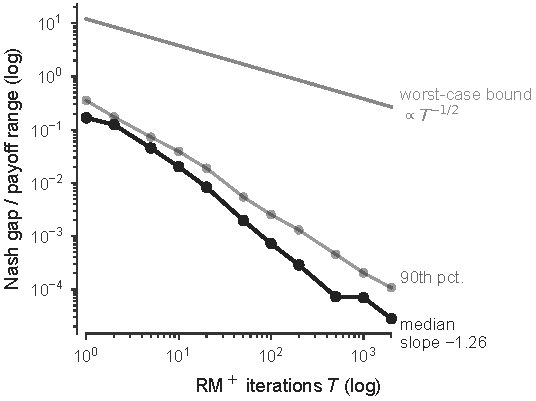
\includegraphics[width=3.58in]{figures/fig_rmplus.pdf}
\caption{RM$^+$ converges far faster than its worst-case $T^{-1/2}$ bound on real stage matrices. Nash gap of the averaged RM$^+$ strategy as a share of the payoff range: median (black) and 90th percentile (gray) over $n=35$ full depth-2 matrices from random mid-game positions. Gray line: median over matrices of the proved bound $2(\sqrt n+\sqrt m)/\sqrt T$. The median slope is fitted for $T\ge10$.}
\label{fig:rmplus}
\end{figure}

% =====================================================================
\section{The regret layer: Hedge over experts}
\label{sec:regret}
The per-turn agent is strong against weak opponents only through its matrix, and deterministic play is exploitable, as the lectures predict for any deterministic rule facing an adversary that knows it (\cref{sec:prelim}). We therefore add Hedge over experts: the experts problem of \cref{sec:prelim} with the real opponent as Nature, in the lectures' adversary model (the opponent may know the algorithm and the mixture $p_t$, but not the sampled action). The goal is the hustler's: exploit when an expert does better, retreat to the equilibrium expert otherwise. Our guarantees are on external regret, and the losses are $l=1-r$ for the rewards $r\in[0,1]$ defined in \cref{sec:setting}. We work under hypothesis (E): at every turn one expert is an $\epss$-equilibrium of $\Ahat_t$ (the RM$^+$ expert).

\begin{lemma}[Hedge with fixed share, pathwise]\label{lem:H}
For any adaptively chosen $r_t\in[0,1]^k$ and every expert $e$, with constant step $\eta$ and share $\alpha$,
$\sum_{t\le S}(r_{t,e}-w_t\cdot r_t)\le\ln k/\eta+\eta S/8+S\ln\tfrac1{1-\alpha}/\eta=:\Reg_S$.
\end{lemma}
This is standard~\cite{FS97,HW98,CBL06}. Only the summation step is in Lean (\texttt{hedge\_telescope}); the per-step Hoeffding inequality enters as a hypothesis and was checked by reading. For X6's constants ($k=3$, $\eta=0.2$, $\alpha=0.002$) the bound is $5.49+0.035\,S$, which is linear in $S$.

\begin{proposition}[safety relative to the surrogate, E1]\label{prop:E1}
Assume (E). On every path and against any opponent:
(a) with the per-turn normaliser $\Delta_t=\range\Ahat_t$, $\sum_{t\le S}\big(p_t\cdot\Ahat_t[:,b_t]-\val\Ahat_t+\epss\big)/\Delta_t\ge-\Reg_S$;
(b) with a fixed normaliser $\Dbar$, $\sum_{t\le S}p_t\cdot\Ahat_t[:,b_t]\ge\sum_{t\le S}(\val\Ahat_t-\epss)-\Dbar\Reg_S$.
\end{proposition}
Lean: \texttt{claim1\_weighted}, \texttt{claim1\_fixed}, \texttt{learner\_reward\_linear}. The raw-unit version of (a) is \emph{false}: alternating $\Ahat$ and $0.01\Ahat$ against an opponent that plays column 2 on high-stakes turns and column 1 on low-stakes turns gives a deficit of $S/3$, verified by brute force. This is why the shipped learner uses $\Dbar=400$. Note that the guarantee is relative to the surrogate $\Ahat_t$, not to win probability.

\begin{lemma}[anytime FTRL as shipped, R2a]\label{lem:R2}
% VERIFIED 2026-11-14
With $\beta_1\ge\beta_2\ge\dots>0$ and $w_t\propto\exp(\beta_tL_{t-1})$, for adaptive rewards in $[0,1]^k$, $\Reg_T\le\ln k/\beta_T+\frac18\sum_t\beta_t$ on every path. For the shipped indexing $\beta_t=\eta_{t-1}$,
\begin{equation}\label{eq:R21}
\Reg_T\;\le\;\tfrac32\sqrt{T\ln k/2}+\sqrt{\ln k/8}.
\end{equation}
\end{lemma}
\begin{proof}[Proof sketch]
Use the potential $\Phi_t(\beta)=\beta^{-1}\ln(\frac1k\sum_ie^{\beta L_{t,i}})$. Each step costs at most $w_t\cdot r_t+\beta_t/8$ (Hoeffding's lemma), and $\Phi_t$ is nondecreasing in $\beta$ (Lyapunov's inequality), so decreasing steps only help. Telescope.
\end{proof}
The textbook anytime bound (\cite{CBL06}, Thm~2.3) uses $\eta_t$ rather than $\eta_{t-1}$ at turn $t$, so it does not literally apply to our code; \eqref{eq:R21} is proved for the code's indexing instead.
Compared with the lectures' MWU, our update is the exponential-weights form $w\propto e^{\beta L}$ with a decreasing step instead of $w\leftarrow w(1-\eta l)$ with a fixed $\eta$ tuned to a known $T$; both have regret of order $\sqrt{T\ln k}$, with constant 2 for MWU and $\frac32/\sqrt2$ for \eqref{eq:R21}. Carried weights make a match one long run of the experts problem ($T$ = all non-forced turns of the match), while reset weights start a short run each game ($T\approx$ one game's length). For $k=2$ the constant $3/2$ is asymptotically attained (the exact worst case is $1.487\sqrt{T\ln 2/2}$ at $T=4\times10^4$).

\begin{theorem}[carried weights, E2$'$]\label{thm:E2p}
% VERIFIED 2026-11-14
Assume (E) in engine units and one \emph{global} calibration $a>0$, $c$ with $\lVert a\Ahat_t+c-\Qstar_t\rVert_\infty\le\epsv^{\rm glob}$ at every learner turn. Let rewards be as coded ($\Dbar=400$, clipped, FTRL step of \cref{lem:R2} carried across games). Then for every match-long opponent $\sigma$, which may be adaptive, see $p_t$ and know the algorithm, in payoff units,
\[
\frac1N\sum_{g=1}^N\big(\Vstar_0(s^g_0)-\E_\sigma[u_g]\big)\le\Hbar_\sigma(a\epss+2\epsv^{\rm glob})+400a\Big(3\sqrt{\tfrac{\Hbar_\sigma\ln k}{8N}}+\tfrac1N\sqrt{\tfrac{\ln k}8}\Big)+\frac{\E_\sigma[C_S]}N,
\]
with clipping loss $C_S=\sum_{t\le S}a(\range\Ahat_t-400)^+$ and $\Hbar_\sigma$ the mean game length against $\sigma$.
\end{theorem}
The proof combines Theorem E2 of our notes (a direct telescoping identity for history-dependent learners, plus \cref{lem:one} per turn; per-turn step in Lean as \texttt{composition\_step}) with \cref{lem:R2} and the affine invariance of \cref{lem:R6a}. It bounds the \emph{average over games}, not the exploitability of any single game's policy. A per-turn calibration would turn the fixed normaliser back into a per-turn one, which is why the calibration must be global. On all six exactly solved endgames the global calibration returns $a\approx0$ ($\le10^{-8}$) and $\max\epsv^{\rm glob}=1.0$, so E2$'$ does not apply (hypothesis $a>0$ fails; as $a\to0^+$ its budget is vacuous) for the heuristic leaf (\cref{sec:leaf} explains why). Explicit counterexample to per-turn calibration: identical $\Ahat$ every turn with $\Qstar=a_t\Ahat$, $a_t$ alternating between $1/200$ and $0.01/200$. Per-turn calibration is exact ($\epsv=\epss=0$), yet the deficit in $\Qstar$ units is 0.248 per turn, linear in $S$. The clipping term $C_S$ is nonzero on turns with $\range\Ahat_t>400$, about 6\% of learner turns (1,922 turns from 44 Hedge games against MCTS at 2,000 iterations; 95\% CI 3--10\%, clustered by game) and 8.5\% of 200 random starting positions. A reward is actually clipped far less often: on 0.5\% of learner turns (95\% CI 0.04--1.4\%) for the opponent's realised move.

\textbf{Exploitation (E3).} On every path the learner's surrogate payoff is at least the best fixed expert's minus $\Dbar\Reg_S$. The comparator, however, is the expert's surrogate payoff \emph{along the learner's own trajectory and against the moves actually made}. That is external regret, not policy regret~\cite{Aro12b}, and not the game payoff of ``always follow expert $e$''.

\begin{proposition}[incremental anytime MW has linear regret, R1]\label{prop:R1}
% VERIFIED 2026-11-14
Let $\lambda_{t+1}=\lambda_t+(c/\sqrt t)\,r_t$, $w_t\propto e^{\lambda_t}$ (our first anytime implementation). With rewards $e_1$ for the first $\lfloor\alpha T\rfloor$ turns and $e_2$ afterwards,
$\lim_{T\to\infty}\Reg_T/T=\kappa(\alpha)=\min(2\alpha,1-2\alpha)^+$, independent of $c$ and $k$. In particular $\kappa(0.3)=0.40$, and the maximum is $\kappa(1/4)=1/2$.
\end{proposition}
\begin{proof}[Proof sketch]
Expert~1's lead after phase 1 is $\approx2c\sqrt{\alpha T}$. Phase 2 erodes it at rate $c/\sqrt t$, so the lead persists until $t\approx4\alpha T$, and the lead is $\Theta(\sqrt T)$, which keeps the weights essentially 0/1. FTRL's sign of $L_{t-1,1}-L_{t-1,2}$ instead flips at $t=2\alpha T$ for any schedule.
\end{proof}
This was a real bug. The shipped learner first coded \texttt{logw += $\eta_t r_t$}, which on a 30/70 phase-switch sequence has regret $0.40\,T$ (measured $0.4001\,T$ at $T=10^4$ on the actual \texttt{Learner}). The FTRL fix \texttt{logw = $\eta_t\cdot$cum} has regret 1.46 at $T=10^3$--$10^5$. All Hedge games reported in \cref{sec:exp} were rerun with the fix. Orabona and P\'al~\cite{OP18} (Thm~4 in the arXiv version) prove $\mathrm{Regret}\ge T/6$ for entropic mirror descent with step $1/\sqrt t$ on the same kind of two-phase sequence (phases $T/3$, $2T/3$). New here: the exact limit $\kappa(\alpha)=\min(2\alpha,1-2\alpha)^+$ for every $\alpha$ ($\kappa(1/3)=1/3$ vs.\ their bound $1/6$), and its independence of $c$ and $k$.

\begin{lemma}[weight dynamics, R3a; $k=2$]\label{lem:R3}
% VERIFIED 2026-11-14
Under the shipped FTRL, after $t$ learner turns: (a) $\ln(w_N/w_F)=\eta_tG_t$; (b) if $d_s\equiv d$, then $w_F=\lgs(-d\sqrt{8\ln2}\sqrt t)$, where $\lgs$ is the logistic function; (c) $p_t\cdot\Ahat_t[:,b_t]=q_{N,t}\cdot\Ahat_t[:,b_t]-400\,w_{F,t}\tilde d_t$, with $\tilde d_t=d_t$ without clipping.
\end{lemma}
So the cumulative surrogate advantage $G_t$ can be read off logged weights. The MCTS share decays like a stretched exponential in turns (log-odds $\propto\sqrt t$, not $t$), and the learner's surrogate deficit to the equilibrium expert is exactly $400\,w_F\tilde d_t$ engine units per turn ($\tilde d_t$ is the clipped gap, equal to $d_t$ without clipping). Because a reset learner restarts at $t=1$ every game, by (b) its $w_F$ falls only to about $\lgs(-0.03\cdot2.35\sqrt{35})\approx0.40$ by the end of a typical game, whereas the carried learner enters the exploiter phase at $w_F\approx0.278$ (seed range 0.232--0.362). The data agree (\cref{sec:exp-hedge}).

\begin{proposition}[bracket on the loss to a white-box exploiter, R3c]\label{prop:R3c}
% VERIFIED 2026-11-14
Let $b_t=\argmin_bp_t\cdot\Ahat_t[:,b]$, let $y^\star_t$ be minimax in $\Ahat_t$, and put $\gamma_{F,t}=\val\Ahat_t-q_{F,t}\cdot\Ahat_ty^\star_t\ge0$ and $\mathrm{gap}_{F,t}=\val\Ahat_t-\min_bq_{F,t}\cdot\Ahat_t[:,b]$. Then $w_{F,t}\gamma_{F,t}\le\val\Ahat_t-p_t\cdot\Ahat_t[:,b_t]\le w_{F,t}\mathrm{gap}_{F,t}+w_{N,t}\epss$.
\end{proposition}
The surrogate loss to a white-box exploiter is therefore linear in the MCTS share. A quantitative lower bound would need $\gamma_F$, which we did not log.

\begin{corollary}[surrogate-to-true transfer, R4]\label{cor:R4}
% VERIFIED 2026-11-14
If $\lVert a\Ahat_t+c-\Qstar_t\rVert_\infty\le\epsv(t)$, then along the realised columns, for any $x_t,q_t$: $\sum_t(x_t-q_t)\cdot\Qstar_t[:,b_t]\ge\sum_t(x_t-q_t)\cdot(a\Ahat_t+c)[:,b_t]-2\sum_t\epsv(t)$. In particular the true trajectory advantage of the equilibrium expert is $\ge400a\,G_t-2\sum_t\epsv(t)$.
\end{corollary}
This is the per-turn transfer step (Lemma~1(i), Lean \texttt{composition\_step}) summed along the trajectory. It certifies a true advantage only if $400a\,d>2\bar\epsv$ per turn, and with $a=0$ on the endgames nothing is certified. ``The learner drifts toward the equilibrium expert'' is therefore a statement about $\Ahat$, whose equilibrium that expert is by construction. The only true-unit evidence is the paired score difference in \cref{sec:exp-hedge}.

% =====================================================================
\section{Measuring exploitability}
\label{sec:measure}
Exact exploitability is out of reach except in small endgames, so we bracket it. Fix a target $\pi$ in score units with $v^\star=1/2$ (seat-swapped pairs make the game symmetric).

\begin{proposition}[valid lower bounds, R5a]\label{prop:R5a}
% VERIFIED 2026-11-14
Let exploiters $X_1,\dots,X_{m_X}$ be legal strategies in the target's information model, fixed before the seeds are drawn, each evaluated on $\nu$ independent pairs with mean exploiter score $\bar Z_j$. Then (1) $\expl(\pi)\ge\E\bar Z_j-v^\star$, and with probability $\ge1-\vartheta$, $\expl(\pi)\ge\bar Z_j-v^\star-\sqrt{\ln(1/\vartheta)/(2\nu)}$; (2) for the best of $m_X$, $\expl(\pi)\ge\max_j\bar Z_j-v^\star-\sqrt{\ln(m_X/\vartheta)/(2\nu)}$; without the $\ln m_X$ term $\max_j\bar Z_j$ is biased upward (winner's curse); (3) re-evaluating the selected exploiter on fresh pairs restores (1) with no $\ln m_X$ term.
\end{proposition}
These are Hoeffding's inequality, a union bound and conditioning, which are textbook. With $m_X$ zero-edge exploiters at $\nu=20$, the winner's-curse bias is $+0.067$ for $m_X=3$ and $+0.121$ for $m_X=10$ (computed for draw-free coin-flip games; with 50\% draws the bias is $+0.047$ / $+0.086$).

\begin{proposition}[what the exploitation gain is, R5b]\label{prop:R5b}
% VERIFIED 2026-11-14
For a same-strength non-exploiting baseline $\beta$, let $\gain=s(\pi,\beta)-s(\pi,X)$. Then $v^\star-s(\pi,X)=[v^\star-s(\pi,\beta)]+\gain$, and $\gain\le\expl(\pi)+\expl(\beta)$. If $s(\pi,\beta)\le v^\star$ the gain is a valid lower bound, but it never exceeds the plain bound $v^\star-s(\pi,X)$. If $s(\pi,\beta)>v^\star$ it is not a lower bound by itself.
\end{proposition}
The gain answers a design question, namely how much of an exploiter's success comes from modelling the target rather than from strength. It reads as exploitability only when $\expl(\beta)\ll\gain$. For the equilibrium bots $\beta=\pi$, so the gain equals the plain bound. For foul-play, whose baseline is equilibrium top move (itself exploitable by $\ge0.325$ at the point estimate (certified at 95\%: 0.051 for one exploiter, 0.005 after selecting among 3), \cref{sec:exp-expl}), at 2,000 it ($s=0.31\le\frac12$) the gain 0.035 is a valid lower bound, but weaker than the plain 0.225, and at 75\,ms ($s=0.65>\frac12$) it certifies nothing, since $\expl(\beta)\gtrsim0.325>\gain$.

\begin{proposition}[bracket, R5c]\label{prop:R5c}
% VERIFIED 2026-11-14
Under full information and the assumptions of \cref{thm:full}, with probability $\ge1-\vartheta$,
$\max_j\bar Z_j-v^\star-\sqrt{\ln(m_X/\vartheta)/(2\nu)}\le\expl(\pi)\le\min\{\tfrac12,\tfrac12\Hbar(\epss+2\epsv)\}$ (score units). Under hidden information the upper side gains the $\etaNL+4\TV$ terms.
\end{proposition}
With $\epsv^{\rm glob}\approx1$ the upper side is the trivial $1/2$. The lower side comes from exploiters of increasing power: the one-turn local best response (LBR), which rebuilds the target's matrix and best-responds in it; a depth-2 white-box search exploiter (\texttt{wb2}); and RL best responses. For a \emph{known, deterministic} target, white-box search is much cheaper than RL (\cref{sec:exp-rl}). RL remains the fallback for black-box or hidden-information targets.

% =====================================================================
\section{The leaf value}
\label{sec:leaf}
\begin{lemma}[affine invariance, R6a]\label{lem:R6a}
% VERIFIED 2026-11-14
For $a>0$, \texttt{rm\_plus}$(aM+c)$ returns the same strategies as \texttt{rm\_plus}$(M)$, (in exact arithmetic; in floating point, outputs on matrices with exact ties can differ at round-off level), so $\epss(aM+c)=a\,\epss(M)$. Hence \cref{thm:full} holds with the per-state budget $a_{t,s}\epss+2\epsv^{\rm cal}(t,s)$, where $\epsv^{\rm cal}=\min_{a\ge0,c}\lVert a\Qhat+c-\Qstar\rVert_\infty$. With $a=0$ this budget is $\ge\range\Qstar$, the trivial per-turn loss.
\end{lemma}

\begin{lemma}[inversions force $a=0$; exact terminals, R6b]\label{lem:R6b}
% VERIFIED 2026-11-14
(1) $\epsv^{\rm cal}(M,Q)\ge\frac12\max\{Q_i-Q_j:M_i\le M_j\}$. (2) $a=0$ is an optimal calibration iff some cell in $\argmax Q$ is scored at or below some cell in $\argmin Q$. (3) If terminal children are scored exactly ($\hat V=u$), then $|\Qhat-\Qstar|(a,\beta)\le\pi_{\rm live}(a,\beta)\,\varepsilon_{\rm live}(s)$, so cells whose children are all terminal are exact.
\end{lemma}
\textbf{Why this matters here.} Through \texttt{pe.id(child,0)} the heuristic scores a terminal child by the winner's remaining material, not as a win. On greattusk vs.\ gholdengo, P1-won terminals score $-50$ to $+185$ while live children span $\pm215$, so a won position can rank below a live one. In MCTS self-play on Random Battles, 18 of 151 two-sided decisions (12\%, all late-game) have a terminal child, and in 15 of them the leaf inverts a win or loss against a live child. By \cref{lem:R6b}(2), a single such pair at the worst cell forces $a=0$, and since the global calibration pools every cell of every state, it forces $a=0$ globally. That is what we observe on all six endgames. The fix is exact $\pm1$ terminals plus a bounded live leaf such as $\tanh(h/160)$, which restores the order. Unlike an affine map, $\tanh$ changes the equilibria, as intended.

\begin{proposition}[non-termination, R6c]\label{prop:R6c}
% VERIFIED 2026-11-14
Consider one live state in which $(E,\cdot)$ ends with $0.3$, $(C,E)$ ends with $0.8$, $(C,C)$ loops, and endless play pays 0. Every $V\in[0.3,0.8]$ is a fixed point of the Shapley operator, and the value is $0.3$. The stationary agent ``always $C$'' is a stage maximin at $\Vstar=0.3$ (stage budget $\delta\equiv0$), yet against ``always $C$'' it never terminates and has exploitability $0.3$. Valuing endless play at $\Vstar$ instead reports $0$. With a turn cap $H$, backward induction is exact and \cref{thm:full} holds with equality, charging the whole $0.3$ to the last turn.
\end{proposition}
This is the Everett / Dubins--Savage phenomenon~\cite{Everett57,DS65,MS96} (an optimal strategy must be thrifty and equalizing in the Dubins--Savage terminology) in the form of \cref{thm:full}; the minimal example and the last-turn attribution are ours. It explains a failed sanity check in our exact endgames (\cref{sec:exp-end}). The 300-turn cap makes the real game finite, but our agents are stationary, so the cap does not remove this exploitability. It only makes the theory account for it.

% =====================================================================
\section{Links to MCTS and RL}
\label{sec:links}
Notation follows \cref{sec:setting}. Let $e_t=V^\star_t(s_t)-\min_bx_t^\top Q^\star_t(s_t)e_b\ge0$ be the stage exploitability of the agent's stage strategy $x_t$ in the true $Q^\star$, and $\ell_t(x,y)=V^\star_t(s_t)-x^\top Q^\star_t(s_t)y$. Let $\sigma_g$ be the myopic $Q^\star$-exploiter (plays $b_t\in\arg\min_bx_t^\top Q^\star_te_b$), $\sigma_{\rm BR}$ a best response, and $\tau\le H$ the first stage at which the game is over (terminal or cap, cap payoff $0$).

\begin{lemma}[potential telescoping, L0]\label{lem:L0}
Let $\Phi_t(h_t)$ be any real function of histories, $t\le H$, with $\Phi=u$ at terminal states and $\Phi_H=0$ for live histories at the cap. Write $Q[\Phi]_t(h,a,b)=\E[\Phi_{t+1}(h')\mid h,a,b]$. Then for all history-dependent $\pi,\sigma$: $\Phi_0(h_0)-V(\pi,\sigma)=\E_{\pi,\sigma}\big[\sum_{t<\tau}(\Phi_t(h_t)-x_t^\top Q[\Phi]_t(h_t)y_t)\big]$.
\end{lemma}
\begin{proof}
On each path $\Phi_0-\Phi_\tau=\sum_{t<\tau}(\Phi_t-\Phi_{t+1})$, and $\Phi_\tau$ is the payoff by the boundary conditions. For $t<\tau$, $a_t\sim x_t$ and $b_t\sim y_t$ are independent given $h_t$ (simultaneous moves; neither side sees the other's realised action this turn; this is the only assumption beyond the boundary conditions), so $\E[\Phi_{t+1}\mid h_t]=x_t^\top Q[\Phi]_ty_t$. Take expectations and apply this term by term; $\tau\le H$, so the sum has at most $H$ terms.
\end{proof}
Each formulation below is \cref{lem:L0} with a different potential.
\begin{center}\small
\begin{tabular}{@{}p{3.6cm}p{9.2cm}p{2.6cm}@{}}
\toprule
Potential $\Phi$ & Reading & Result \\
\midrule
$V^\star$ (game value) & exploitability = expected sum of per-turn losses to the value & L1 (Theorem A), L2 \\
$V^{\pi,\sigma_k}$ (current opponent policy in the MDP $M_\pi$) & performance-difference lemma, the engine of policy-gradient / NPG analyses & L3 \\
$\hat V$ (learned or heuristic leaf) & exploitability bounded by the minimax TD (Bellman) residual & L6 \\
\bottomrule
\end{tabular}
\end{center}

\begin{theorem}[identity and sandwich, L1]\label{thm:L1}
(a) For all $\pi,\sigma$: $V^\star_0(s_0)-V(\pi,\sigma)=\E_{\pi,\sigma}[\sum_{t<\tau}\ell_t(x_t,y_t)]$; hence $\expl(\pi)=\sup_\sigma\E_{\pi,\sigma}[\sum_{t<\tau}\ell_t]$.
(b) $\E_{\pi,\sigma_g}[\sum_{t<\tau}e_t]\le\expl(\pi)\le\E_{\pi,\sigma_{\rm BR}}[\sum_{t<\tau}e_t]$.
(c) If $e_t\le\epss+2\epsv$ at every live state, the upper side is $\le\Hbar(\epss+2\epsv)$, i.e.\ Theorem A.
\end{theorem}
\begin{proof}
(a) is \cref{lem:L0} with $\Phi=V^\star$. (b) Under $\sigma_g$, $\ell_t=e_t$, and $\expl(\pi)\ge V^\star_0-V(\pi,\sigma_g)$. For the upper side, $\expl(\pi)=\E_{\pi,\sigma_{\rm BR}}[\sum\ell_t]$ by (a), and $\ell_t(x,y)\le e_t$ pointwise; $e_t\ge0$ because $\min_bx^\top Q^\star e_b\le\val Q^\star=V^\star_t$. (c) $\E[\sum e_t]\le(\epss+2\epsv)\E[\tau]$.
\end{proof}
\begin{remark}[Example L1b: the gap can be $2-\delta$]
Let $H\ge2$. At $s_0$ the agent is forced and the opponent has two actions: $b_1$ ends the game with payoff $1-\delta$ ($0<\delta<1$); $b_2$ moves deterministically to $s_1$, where the agent has a safe row paying $+1$ against every column and a bad row paying $+1/-1$, and plays the bad row. Then $V^\star(s_1)=1$, $Q^\star_0(s_0)=(1-\delta,1)$, $V^\star_0=1-\delta$, $e_0=0$. $\sigma_g$ picks $b_1$, so the lower side is $0$; $\sigma_{\rm BR}$ plays $b_2$ and then the $-1$ column, so $\expl=2-\delta$, while the upper side is $e_0+e_1=2$. (Matching pennies at $s_1$ with $b_1$ paying $-\delta$ gives only $1-\delta$, half the range.)
\end{remark}
\emph{Prior art.} With a trivial opponent (a) is the performance-difference lemma of Kakade \& Langford~\cite{KL02} (their Lemma~6.1). The upper side has discounted precedents: Wei et al.~\cite{Wei21} (Lemma~32) bound the duality gap by $\frac2{1-\gamma}\max_s$ of the $Q^\star$-stage gap, and Daskalakis, Foster \& Golowich~\cite{DFG20} (Lemma~3) give a Markov-game performance-difference lemma. Ours is the finite-horizon, trajectory-weighted refinement; the exact identity (a) and the myopic lower side with Example L1b were not found in the papers read (not a proof of novelty).

\begin{theorem}[Hedge with an equilibrium expert is safe in the full game, L2]\label{thm:L2}
\emph{Setting (idealised \texttt{exp3\_live.Learner}).} $G$ games are played in sequence against an opponent that may adapt within and across games and may see the learner's mixture $p_i$ before it moves, \emph{but not the realised action $a_i$} (the adversary model of \cref{sec:prelim}) (an opponent that sees $a_i$ breaks (b) in simulation). Turns are numbered globally $i=1,\dots,T$, $T\le GH$ random. At turn $i$ the learner sees $\Ahat_i\in[-1,1]^{n\times m}$ (clipped to the payoff range, so $\lVert\Ahat_i-Q^\star_{t_i}(s_i)\rVert_\infty\le\epsv$) and $k$ expert strategies $q_{e,i}$, and plays $p_i=\sum_ew_{e,i}q_{e,i}$ with $w_i$ anytime-FTRL Hedge on the \emph{normalised} past rewards $(q_{e,j}^\top\Ahat_je_{b_j}+1)/2\in[0,1]$. This gives pathwise regret $\sum_{i\le T}(q_{e,i}-p_i)^\top\Ahat_ie_{b_i}\le R(T)=2\big(1.5\sqrt{T\ln k/2}+\sqrt{\ln k/8}\big)$. Let $\hat\ell_i(q,b)=\val(\Ahat_i)-q^\top\Ahat_ie_b$. Then
(a) $\E[\sum_{g=1}^G(V^\star_0(s^g_0)-u_g)]\le\E[\min_e\sum_{i\le T}\hat\ell_i(q_{e,i},b_i)]+\E[R(T)]+2\epsv\E[T]$.
(b) \emph{Safety.} If some expert is $\epss$-optimal in every $\Ahat_i$, then $\E[\sum_g(V^\star_0-u_g)]\le(\epss+2\epsv)\E[T]+\E[R(T)]$; the average per-game loss is $\le\bar L(\epss+2\epsv)+\E[R(T)]/G$ with $\bar L=\E[T]/G$.
(c) \emph{Exploitation.} $\E[\sum_g(u_g-V^\star_0)]\ge\E[\max_e\sum_i(-\hat\ell_i(q_{e,i},b_i))]-\E[R(T)]-2\epsv\E[T]$.
(d) Resetting the weights each game replaces $R(T)$ by $\sum_gR(T_g)$; since $\sum_g\sqrt{T_g}\ge\sqrt{\sum_gT_g}$, the persistent bound is smaller (a comparison of bounds, not of outcomes).
\end{theorem}
\begin{proof}[Proof sketch]
Apply \cref{thm:L1}(a) to each game with $x=p_i$; replace $Q^\star$ by $\Ahat_i$ at cost $2\epsv$ per turn (val is 1-Lipschitz in sup-norm); apply the pathwise regret bound and take $\min_e$, then expectations. (b) uses $\hat\ell_i(q_{e^\star,i},b)\le\epss$; (c) negates the steps; (d) applies the bound per game. Forced turns have $\ell_i\le0$, so omitting them from $T$ keeps the bounds valid.
\end{proof}
\emph{Prior art.} The idea is known: Ganzfried \& Sandholm~\cite{Gan15} (\S6.4) note that no-regret selection between an equilibrium and an exploiter is ``safe in the limit'' but not in finitely repeated games (their safety definition requires zero slack per period). What L2 adds is the quantified finite-sample slack $R(T)+2\epsv\E[T]$, the extension to stochastic games with a leaf through L1, and (d).
\begin{remark}[L2.1: experts in every state]
With the pure actions as experts and separate weights per state $(t,s)$, (a) and (c) are unchanged (regret $\sum_sR(T_s)$). With one shared fixed $\eta$ this is Hedge over all Markov policies: $\ln|\Pi|=|S|\ln n$ versus $\ln k$ for our tied 3-expert mixture. This per-state Hedge is Even-Dar, Kakade \& Mansour~\cite{EKM09}, and the NPG update is the same per-state Hedge on advantages~\cite{Aga21}.
\end{remark}

\begin{theorem}[an RL best response is per-state Hedge in $M_\pi$, L3]\label{thm:L3}
Fix a Markov agent $\pi$; the opponent faces the finite-horizon MDP $M_\pi$. Let $\sigma_{k+1}(b\mid t,s)\propto\exp(-\eta\sum_{j\le k}\hat Q^{\sigma_j}_t(s,b))$ with critic error $\varepsilon_k(t,s)=\max_b|\hat Q^{\sigma_k}_t(s,b)-Q^{\sigma_k}_t(s,b)|$ and $\hat Q$ clipped to $[-1,1]$, and let $d^\circ_t(s)=P_{\pi,\sigma^\circ}(s_t=s,t<\tau)$ for a comparator $\sigma^\circ$, so $\sum_{t,s}d^\circ_t(s)=\Hbar(\sigma^\circ)$. For every Markov comparator, in particular a Markov best response,
\[\tfrac1K\sum_{k=1}^KV(\pi,\sigma_k)-V(\pi,\sigma^\circ)\le\sum_{t,s}d^\circ_t(s)\tfrac{\Reg_K(t,s)}{K}+\tfrac2K\sum_k\sum_{t,s}d^\circ_t(s)\varepsilon_k(t,s),\]
with $\Reg_K(t,s)\le\frac{\ln|B(s)|}\eta+\frac{\eta K}2$; with $m=\max_s|B(s)|$ and $\eta=\sqrt{2\ln m/K}$ the first term is $\le\Hbar(\sigma^\circ)\sqrt{2\ln m/K}$.
\end{theorem}
\begin{proof}[Proof sketch]
\Cref{lem:L0} in $M_\pi$ with $\Phi=V^{\sigma_k}$ and opponent $\sigma^\circ$ gives $V(\pi,\sigma_k)-V(\pi,\sigma^\circ)=\sum_{t,s}d^\circ_t(s)\langle\sigma_k(s)-\sigma^\circ(s),Q^{\sigma_k}_t(s,\cdot)\rangle$. The weights $d^\circ$ do not depend on $k$, so averaging over $k$ gives per-state Hedge regret against the fixed $\sigma^\circ(s)$; the critic costs $2\varepsilon_k$ per term.
\end{proof}
This is the finite-horizon form of~\cite{EKM09,Aga21}; what is ours is the horizon factor, the comparator's expected game length $\Hbar$, the same as in Theorem~A.
\emph{L3b (distribution mismatch).} If the critic is fit on-policy with $\sum_sd^{\sigma_k}_t(s)\varepsilon_k(t,s)\le\varepsilon_{\rm crit}$ and $C=\max_{k,t,s}d^{\rm BR}_t(s)/d^{\sigma_k}_t(s)$, the critic term with $\sigma^\circ=\sigma_{\rm BR}$ is $\le2HC\varepsilon_{\rm crit}$; $C$ is large exactly when the BR's exploiting line is one the learner rarely visits. It is the analogue of the transfer step in Agarwal et al.~\cite{Aga21} (Cor.~6.1) and Kakade \& Langford~\cite{KL02}.
\emph{L3c (undirected exploration).} On a chain $s_0\to\dots\to s_D$ where only action $b^\star_j$ at $s_j$ continues (every other action ends the game with payoff $0$) and $s_D$ is matching pennies against a $\pi$ that plays pure heads, $\expl(\pi)=1$, yet any exploiter whose per-state policy stays uniform while all observed returns are equal (per-state Hedge/NPG/PPO with a Monte-Carlo critic and no exploration bonus) never reaches $s_D$ in its first $N$ games with probability $\ge1-N|B|^{-D}$, while backward induction in $M_\pi$ (white-box, as \texttt{wb2}) finds the gain-1 response with $O(D|B|)$ work and no games. This is an instance of the classical undirected-exploration lower bounds of Whitehead~\cite{Whi91} (Thm~8, Cor.~9) and Kakade~\cite{Kak03} (\S4.3). Optimistic tabular RL needs only $\mathrm{poly}(D,|B|)$ games here, and exact-critic Hedge does not satisfy the hypothesis.

\begin{proposition}[exact identity for visit shares, L4]\label{prop:L4}
At one MCTS node on the engine's scale, side one maximises $\Ahat\in[0,1]^{n\times m}$ and side two maximises $1-\Ahat$; simulation $i$ picks $(a_i,b_i)$ and returns $r_i$ with $\E[r_i\mid\text{past},a_i,b_i]=\Ahat(a_i,b_i)$. With visit shares $\bar x_N,\bar y_N$ and mean-reward external regrets $\mathrm{Reg}^1_N,\mathrm{Reg}^2_N$,
$\max_a(\Ahat\bar y_N)_a-\min_b(\bar x_N^\top\Ahat)_b=(\mathrm{Reg}^1_N+\mathrm{Reg}^2_N)/N.$
\end{proposition}
\begin{proof}
$\sum_i\Ahat(a,b_i)=N(\Ahat\bar y_N)_a$ and $\sum_i\Ahat(a_i,b)=N(\bar x_N^\top\Ahat)_b$; adding the two regrets cancels the realised joint terms.
\end{proof}
This is the inequality of \cref{prop:selfplay} holding with equality, for exact regrets. Our RM$^+$ average and MCTS visit shares are thus the same object, the average strategy of no-regret self-play on a stage matrix, with full-information versus bandit feedback; UCB1, however, is a stochastic-bandit rule with no regret guarantee against an adaptive opponent, so the hypothesis of \cref{prop:selfplay} is not supplied; both feed Theorem~A through the stage gap. The visit shares converge iff $\mathrm{Reg}^1_N+\mathrm{Reg}^2_N=o(N)$ (sublinear on each side is sufficient, not necessary: decoupled UCB1 on matching pennies has gap $0$ while $\mathrm{Reg}^2_N/N=+\frac12$). For deeper trees, Lis\'y et al.~\cite{Lis13} (Thm~4.11) prove almost-sure convergence to a subgame-perfect equilibrium (quadratic in depth, no rate) for Hannan-consistent selection in the mean-propagating variant of SM-MCTS on a complete tree with exact terminals, and Kova\v{r}\'ik \& Lis\'y~\cite{KL19} (Thm~4.1) show plain SM-MCTS with Hannan-consistent selection can converge outside the $1/5$-Nash set. None of this covers poke-engine (raw returns, UCB1, heuristic leaf), and no formal DUCT non-convergence proof was found.

\begin{proposition}[decoupled UCB1 can stay uniform, L4b]\label{prop:L4b}
Let $\Ahat\in[0,1]^{n\times n}$ satisfy $\Ahat(a,b)+\Ahat(b,a)=1$, both sides listing options in the same order. Run the code's rule (UCB $\bar r+\sqrt{2\ln N/n}$, unvisited options at $+\infty$, ties to the first index) with deterministic rewards $r_i=\Ahat(a_i,b_i)$. Then $a_i=b_i$ for every $i$, every option's mean stays $\frac12$, and play is round-robin, so $\bar x_N=\bar y_N$ is exactly uniform whenever $n\mid N$. On $\Ahat=[[.5,.9],[.1,.5]]$, where row~0 is dominant, the Nash gap is $0.4$ for every even $N$.
\end{proposition}
\begin{proof}
Induction on $i$ with hypothesis that both sides have identical (count, total) statistics per option. Identical statistics give identical UCB vectors and the same tie rule, so $a_i=b_i=c$; symmetry gives $\Ahat(c,c)=\frac12$, credited as $\frac12$ to each side, so the statistics stay identical and every visited mean is $\frac12$. With equal means UCB decreases in $n_i$ and unvisited options are at $+\infty$, so the pick is the least-visited option (first index on ties): round-robin. For the $2\times2$ example $\Ahat\bar y=(.7,.3)$ and $\bar x^\top\Ahat=(.3,.7)$, gap $.4$.
\end{proof}
The proposition is knife-edge (Bernoulli or $\sigma=0.02$ Gaussian noise breaks the lockstep, and this $2\times2$ then converges, gap about $10^{-4}$ at $10^6$). The non-convergence on generic matrices is numerical only (\texttt{lk4\_duct.py}): in a one-node, depth-1 model with a fixed leaf and exactly poke-engine's selection rule (200 random $3{\times}3$, $5{\times}5$, $10{\times}10$ matrices, biased RPS, matching pennies; $N\le10^6$), with deterministic or low-noise rewards (Gaussian $\sigma\le0.1$) on games with a mixed equilibrium the median Nash gap at $N=10^6$ is $0.10$--$0.25$ and grows with $N$, whereas Hannan-consistent selection on the same matrices (Exp3, bandit regret matching) reaches median gaps of $0.002$--$0.013$ and full-information RM reaches $0.0004$. Pure saddles converge under every noise model. With Bernoulli rewards the gap shrinks slowly (medians at $10^6$: $0.008/0.024/0.043$ for $3{\times}3/5{\times}5/10{\times}10$). \emph{Scope:} this is a model result; Bernoulli rewards converge slowly, and the engine's own noise regime and its real iteration count $N$ are unmeasured; it does not include deeper-tree drift or foul-play's world sampling. The foul-play move rule (keep moves with share $\ge0.75\times$ the top share, sample proportionally) has a floor even on an exact Nash $x^\star$: median exploitability $0.143$ on biased RPS, $0$ on rand3, $0.083$ on rand5 and $0.198$ on rand10 (engine scale $[0,1]$).

\begin{theorem}[what depth buys with exact terminals, L5]\label{thm:L5}
Let the depth-$D$ lookahead use exact val at inner nodes, exact payoffs at terminals and the cap, and a leaf $\hat V$ with $|\hat V-V^\star|\le\varepsilon_{\rm leaf}$ at live frontier states. Define $\rho_0(t,s)=\mathbb 1[s\text{ live},t<H]$ and, for live $s$ and $t<H$, $\rho_D(t,s)=\max_{a,b}\E[\rho_{D-1}(t+1,s')\mid s,a,b]$ ($\rho_D=0$ otherwise). Then $|V^D_t(s)-V^\star_t(s)|\le\varepsilon_{\rm leaf}\rho_D(t,s)$ and $\lVert Q^{(D)}_t(s)-Q^\star_t(s)\rVert_\infty\le\varepsilon_{\rm leaf}\rho_D(t,s)$; hence Theorem~A holds with the per-state budget $\epss+2\varepsilon_{\rm leaf}\rho_D(t,s)$.
\end{theorem}
\begin{proof}
Induction on $D$: each cell satisfies $|Q^{(D)}-Q^\star|\le\E|V^{D-1}_{t+1}-V^\star_{t+1}|\le\varepsilon_{\rm leaf}\E[\rho_{D-1}(t+1,s')]\le\varepsilon_{\rm leaf}\rho_D(t,s)$ after the max over cells, and val is 1-Lipschitz in sup-norm.
\end{proof}
In the middle game both players can usually prolong the game, so $\rho_D\approx1$ and depth alone does not shrink the leaf term; undiscounted termination plays the role that $\gamma$ plays in ADP error-propagation bounds.

\begin{theorem}[minimax TD residual bounds exploitability, L6]\label{thm:L6}
Let $\hat V_t(s)$ be a leaf with exact terminals and $\hat V_H=0$, let the agent play $x_t(s)$ $\epss$-optimal in $Q[\hat V]_t(s)$, and let $\delta_t(s)=\hat V_t(s)-\val Q[\hat V]_t(s)$ be the signed minimax TD residual. Let $\pi^\star$ play maximin-optimal stage strategies of $Q^\star$ and $\hat\sigma$ minimax-optimal ones of $Q[\hat V]$. Then
\[\expl(\pi)\le\E_{\pi,\sigma_{\rm BR}}\Big[\sum_{t<\tau}(\delta_t+\epss)\Big]-\E_{\pi^\star,\hat\sigma}\Big[\sum_{t<\tau}\delta_t\Big]\le\sum_{t<H}\big(2\sup_s|\delta_t(s)|+\epss\big).\]
\end{theorem}
\begin{proof}
\Cref{lem:L0} with $\Phi=\hat V$, twice. Agent side: $\hat V_0-V(\pi,\sigma_{\rm BR})\le\E_{\pi,\sigma_{\rm BR}}[\sum(\delta_t+\epss)]$, since $x^\top Q[\hat V]y\ge\val Q[\hat V]-\epss=\hat V_t-\delta_t-\epss$. Value side: $V^\star_0\le V(\pi^\star,\hat\sigma)$, and $x^{\star\top}Q[\hat V]\hat y\le\val Q[\hat V]=\hat V_t-\delta_t$ gives $V^\star_0-\hat V_0\le-\E_{\pi^\star,\hat\sigma}[\sum\delta_t]$. Add; the sup form follows from $\tau\le H$.
\end{proof}
\begin{remark}[mis-scored terminals]
Let $m=\hat V-u$ on terminal states, with $Q[\hat V]$, $\delta$, the agent and $\hat\sigma$ all built from the mis-scored $\hat V$. Then the bound of \cref{thm:L6} gains $+\E_{\pi,\sigma_{\rm BR}}[m(s_\tau)]-\E_{\pi^\star,\hat\sigma}[m(s_\tau)]$; the second terminal term enters with a \emph{minus} (adding both with a plus fails in 419 of 1000 random games), and the sup form adds at most $2\sup|m|$.
\end{remark}
\emph{Prior art.} The closest published statements are discounted: P\'erolat et al.~\cite{Per16} (Thm~1) for zero-sum Markov games, and Singh \& Yee (1994) for MDPs. L6 is the finite-horizon, undiscounted, signed, exact-trajectory-weight analogue, with termination playing the role of $\gamma$; it is incomparable with Theorem~A (L6 is linear in the residual, whereas Theorem~A with $\epsv\le\sum_{u>t}\sup|\delta_u|$ can be quadratic in $H$; if $\lVert\hat V-V^\star\rVert_\infty=\varepsilon$ then $|\delta|\le2\varepsilon$ and L6 gives $4H\varepsilon$ against $2H\varepsilon$), so use the smaller. \emph{Measured diagnostic} (20 games, our agent vs.\ \texttt{mcts\_policy(2000)}, leaf $\tanh(\text{mid}/k)$ with exact terminals, 651 non-forced states; a probe run, not re-verified): the bound is vacuous, with median $2\sum_t|\delta_t|=4.2$ per game against a payoff range of $2$; the mean-$\delta^2$ minimiser is $k\approx320$--$400$ versus our $k=160$ (0.0073 vs.\ 0.0043).

\begin{center}\small
\begin{tabular}{@{}p{2.2cm}p{3.6cm}p{4.6cm}p{4.4cm}@{}}
\toprule
 & Our per-turn agent & MCTS (poke-engine, foul-play) & RL best response (PPO) \\
\midrule
Regret minimised at & current turn's stage matrix & every tree node, each side separately & every state (shared via the policy net) \\
Learner, feedback & RM$^+$, full information, adversarial guarantee & UCB1 per side, bandit feedback, stochastic-bandit guarantee only (shares need not converge: L4) & Hedge on advantages (NPG; PPO approximates it) \\
Output & linear average of RM$^+$ iterates & visit shares, then the $0.75$-threshold rule & current policy \\
Regret $\to$ gap & folk theorem & exact identity L4 & PDL, L3 \\
Potential in L0 & $V^\star$ (L1) & $V^\star$ (L1) & $V^{\pi,\sigma_k}$ (L3) \\
Error more iterations do not remove & leaf: $2\epsv$ per turn & frontier leaf $2\varepsilon_{\rm leaf}\rho_D$ (L5) & critic error under the BR's distribution, $\times C$ (L3b) \\
Horizon factor & $\Hbar$ vs.\ BR & same & $\Hbar(\sigma_{\rm BR})$ \\
\bottomrule
\end{tabular}
\end{center}

{\sloppy\textbf{Verification.} The proofs were checked by adversarial reading and by exact brute force on random small games (\texttt{theory/checks/\allowbreak lk1\_telescoping.py}, \allowbreak\texttt{lk2\_safe\_hedge.py}, \allowbreak\texttt{lk3\_rl\_hedge.py}, \allowbreak\texttt{lk4\_duct.py}, \allowbreak\texttt{lk5\_depth.py}, \allowbreak\texttt{lk6\_residual.py}); they are not Lean-checked. The DUCT non-convergence on generic matrices is a numerical finding, not a theorem.\par}

% =====================================================================
\section{Experiments}
\label{sec:exp}
\textbf{Setup.} We used poke-engine 0.0.48 (Rust, Gen~9 with Terastallization) and Showdown's published Gen~9 Random Battle set data (509 species, 873 roles). Our sampler approximates Showdown's generator and skips constraints such as guaranteed same-type attacks. Games come in pairs with the same teams and seed and sides swapped. Score is wins plus $\frac12$ draws, 95\% CIs are taken over pairs, and the 300-turn cap counts as a draw. ``MCTS'' is poke-engine MCTS (most-visited move) at 2,000 iterations unless a time budget is given. ``Foul-play'' reproduces foul-play's selection rule on one world under full information. Unless stated otherwise, the experiments in this section use full information.

\subsection{Strength: MCTS vs.\ equilibrium play at matched time}
\label{sec:exp-strength}
\begin{table}[h]
\centering\small
\caption{Head-to-head scores of A vs.\ B (E7, E7t; 100 games each).}
\label{tab:strength}
\begin{tabular}{@{}llccc@{}}
\toprule
A & B & Score & 95\% CI & ms/move A / B \\
\midrule
foul-play, 2,000 it & MCTS, 2,000 it (sanity check) & 0.505 & [0.417, 0.593] & 2.9 / 2.8 \\
foul-play, 2,000 it & Equilibrium, sampled & 0.490 & [0.399, 0.581] & 2.8 / 75 \\
foul-play, 2,000 it & Equilibrium, top move & 0.310 & [0.235, 0.385] & 2.8 / 74 \\
foul-play, 75 ms (time-matched) & Equilibrium, top move & \textbf{0.650} & [0.571, 0.729] & 72 / 71 \\
foul-play, 75 ms (time-matched) & Equilibrium, sampled & \textbf{0.760} & [0.677, 0.843] & 70 / 61 \\
\bottomrule
\end{tabular}
\vspace{-0.6em}
\end{table}
At equal time, foul-play-style MCTS beats equilibrium play clearly. This agrees with the earlier X1 run, in which time-matched MCTS (75\,ms) beat equilibrium top move 0.345 [0.289, 0.401] and safest move 0.263 [0.210, 0.315], whereas at 2,000 MCTS iterations (25$\times$ less time) the equilibrium bots won. The matrix builder is Python and MCTS is Rust, so part of the gap is implementation speed. The rest is consistent with the leaf term dominating~\eqref{eq:headline}.

\subsection{Exploitability}
\label{sec:exp-expl}
\begin{table}[h]
\centering\small
\caption{Target vs.\ its one-turn LBR exploiter (score of the target; 60 games $=$ 30 pairs each), and exploitation gain (\cref{prop:R5b}). Gains come from different experiments and are indicative.}
\label{tab:lbr}
\begin{tabular}{@{}lcccc@{}}
\toprule
Target & vs.\ LBR [95\% CI] & vs.\ same-strength non-exploiter & Gain & Gain 95\% CI \\
\midrule
foul-play, 2,000 it (2.8 ms) & 0.275 [0.161, 0.389] & 0.310 & 0.035 & [$-0.10$, 0.17] \\
foul-play, 75 ms & 0.533 [0.437, 0.629] & 0.650 & 0.117 & [$-0.01$, 0.24] \\
Equilibrium, top move & 0.317 [0.232, 0.401] & 0.5 & \textbf{0.183} & [0.10, 0.27] \\
Equilibrium, sampled & 0.475 [0.377, 0.573] & 0.5 & 0.025 & [$-0.07$, 0.12] \\
MCTS, 2,000 it (most visited) & 0.258 [0.166, 0.351] & 0.419 (cross-experiment) & \textbf{0.160} & [0.06, 0.26] \\
\bottomrule
\end{tabular}
\vspace{-0.6em}
\end{table}
An LBR score mixes exploitation with strength, because LBR is itself a depth-2 matrix bot. Our earlier reading that ``foul-play is as exploitable as plain MCTS'' was confounded: at 2,000 iterations LBR mainly wins by being the stronger bot. Only three effects are significant (\cref{fig:exploit}): the gain against top move ($z=4.3$), the gain against plain MCTS ($z=3.1$), and the top-move minus sampled difference (0.158 [0.03, 0.29]). Foul-play's lower gain is suggestive ($z=1.45$ vs.\ plain MCTS) and depends on the baseline: with equilibrium sampled as baseline its gains become 0.21--0.23. By \cref{prop:R5b}, at 2,000 it the foul-play gain is a valid but weak lower bound, and at 75\,ms it certifies nothing about foul-play's exploitability. Against LBR, the deterministic equilibrium bot loses about 0.18 while equilibrium sampling is indistinguishable from 0.5, which is the robustness side of the trade-off.
% FIGURE: scatter of score vs. time-matched opponent (strength) against exploitation gain (robustness), one point per bot with CI whiskers.
\begin{figure}[t]
\centering
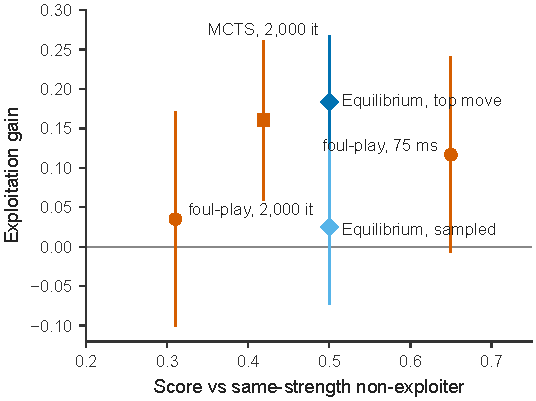
\includegraphics[width=3.58in]{figures/fig_exploit.pdf}
\caption{Only the deterministic bots, equilibrium top move and plain MCTS, show a significant exploitation gain. One point per bot: score against a same-strength non-exploiter (0.5 by symmetry for the equilibrium bots) and exploitation gain (that score minus the score against the bot's LBR exploiter). Bars: 95\% CIs over seat-swapped pairs (30 LBR pairs per bot; 50 or 200 baseline pairs). Gains come from different experiments (\cref{tab:lbr}).}
\label{fig:exploit}
\end{figure}

\textbf{White-box search exploiter (W1).} \texttt{wb2} knows the target's exact policy. For its top-$K$ actions it expands chance branches and best-responds to the target one turn deeper. W1 uses 100 pairs (200 games) per target on fresh seeds disjoint from all earlier runs, with the same pruning in both cells: top $K{=}4$ own actions, 80\% target support, chance branches to 95\% mass. A 10--20-pair pilot had suggested that sampled play is as exploitable as top move.
\begin{table}[h]
\centering\small
\caption{White-box exploiter wb2 (W1; exploiter's score). Lower bound $=$ score $-0.5$ (point estimate); LCB is Hoeffding at 95\% for one pre-registered exploiter (\cref{prop:R5a}, $m_X{=}1$).}
\label{tab:wb}
\begin{tabular}{@{}lcccccc@{}}
\toprule
Target & Pairs & Score & 95\% CI & Point LB & LCB & W-L-D (cap draws) \\
\midrule
Equilibrium, top move & 100 & 0.873 & [0.836, 0.909] & 0.373 & 0.250 & 160-11-29 (29) \\
Equilibrium, sampled & 100 & 0.713 & [0.654, 0.771] & 0.213 & 0.090 & 136-51-13 (13) \\
\bottomrule
\end{tabular}
\vspace{-0.6em}
\end{table}
Top move minus sampled is $+0.160$ [$+0.091$, $+0.229$]; the seeds are disjoint, so the cells are independent. Top move is clearly more exploitable, so sampling buys robustness against a depth-2 white-box exploiter as well as against one-turn LBR. This is the lectures' point that an adversary who knows a deterministic algorithm can predict its action (\cref{sec:prelim}): the white-box exploiter knows the target's policy, so against top move it faces a known pure action, while against sampled play it sees only the mixture. Both targets have certified positive lower bounds (Hoeffding radius $\sqrt{\ln 20/200}=0.122$; one pre-registered exploiter, so no selection correction): at least 0.250 for top move and 0.090 for sampled. This is the lower side of the bracket; the upper side stays vacuous. Caveat: the 80\% support truncation affects only the sampled cell, since the argmax target has a single support action, so part of the gap may come from pruning. A $K{=}5$/95\% rerun of the sampled cell would separate the two. Wall time was 59 min on 5 local processes.

\textbf{Hidden information (X5).} An exploiter that knows the agent-form algorithm and the true state (one turn deep) gained 0.00 against sampled play and 0.03 against top-move play relative to the Oracle control (40 games each, CIs about $\pm0.13$--$0.16$). This is inconclusive, not zero. Even top-move play depends on which 4 worlds the agent samples, which the exploiter cannot reproduce.

\subsection{Hedge over \{MCTS, equilibrium\}}
\label{sec:exp-hedge}
\begin{table}[h]
\centering\small
\caption{Hedge2 (\{foul-play MCTS, equilibrium sampled\}), fixed FTRL update. Top: weights reset each game (H1 rerun). Bottom: weights carried vs.\ reset on the same game seeds, 4 seeds $\times$ (30 games vs.\ MCTS, then 30 vs.\ the white-box exploiter that knows $p_t$). H1 rows: CIs over pairs; carried/reset rows: CIs over 4 seeds ($t_3$).}
\label{tab:hedge}
\begin{tabular}{@{}llcccc@{}}
\toprule
Weights & Opponent & Games & Score & 95\% CI & MCTS-expert weight (end of game, mean over games) \\
\midrule
Reset (H1) & MCTS, 2,000 it & 100 & 0.560 & [0.473, 0.647] & 0.46 \\
Reset (H1) & white-box exploiter & 60 & 0.408 & [0.294, 0.522] & 0.38 \\
\midrule
Carried & MCTS, 2,000 it & 120 & 0.533 & [0.355, 0.712] & 0.34 \\
Carried & white-box exploiter & 120 & 0.533 & [0.441, 0.625] & 0.14 \\
Reset & MCTS, 2,000 it & 120 & 0.471 & [0.401, 0.541] & 0.45 \\
Reset & white-box exploiter & 120 & 0.388 & [0.308, 0.467] & 0.38 \\
\bottomrule
\end{tabular}
\vspace{-0.6em}
\end{table}
Paired on (seed, game), carried minus reset is $+0.062$ [$-0.050$, $+0.175$] against MCTS and $\mathbf{+0.146}$ [$+0.039$, $+0.253$] against the exploiter. Carrying weights costs nothing detectable against MCTS and makes the learner significantly harder to exploit. The MCTS-expert weight drifts slowly against MCTS (0.45 $\to$ 0.28 over 30 games), then falls faster once the exploiter starts (0.28 $\to$ 0.07; \cref{fig:hedge}). \Cref{lem:R3} accounts for this quantitatively. Fitting $G_t$ linearly per phase gives $d_1=0.0133\pm0.0023$ (vs.\ MCTS) and $d_2=0.0291\pm0.0014$ (vs.\ exploiter) per turn ($\pm$ is the sd over seeds), with $R^2$ between 0.861 and 0.987, and the constant-slope model predicts the logged $w_F$ trajectory within 0.01 at the tabulated games (max error 0.017 over all 60 games, RMS 0.006; slopes fitted in-sample; \cref{tab:r3b}). The estimated per-turn surrogate deficit to the equilibrium expert is 0.0040 (carried) vs.\ 0.0116 (reset) against the exploiter (the persistent regret bound covers both phases, while the realised 0.0040 is exploiter-phase only), a ratio of 2.9, and 0.0043 vs.\ 0.0051 against MCTS, a ratio of 1.2. This matches the sign and asymmetry of the paired score differences. Three caveats apply. (i) Both experts are rewarded under $\Ahat$, which favours the equilibrium expert by construction (\cref{cor:R4}). (ii) The surrogate explanation holds on average but does not predict per-game outcomes (correlation $-0.17$, $n=120$). (iii) The hypothesis that the exploiter's edge grows with the MCTS share is not supported (coefficient $0.0002\pm0.014$). With the buggy incremental update (\cref{prop:R1}), the carried learner had collapsed onto the equilibrium expert within about 10 games and the carried-minus-reset difference was $-0.10$ against MCTS. That was an artefact of the bug.
% FIGURE: MCTS-expert weight w_F vs. game index (carried, per seed + mean) with the constant-slope R3a(b) prediction overlaid; vertical line at the MCTS->exploiter switch.
\begin{figure}[t]
\centering
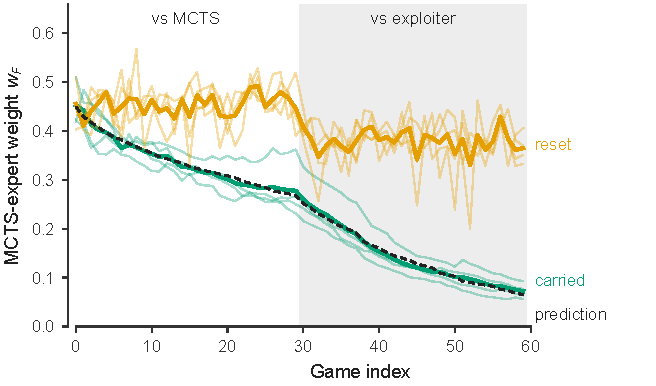
\includegraphics[width=4.38in]{figures/fig_hedge.pdf}
\caption{Carried weights move steadily off the MCTS expert, faster once the exploiter starts, while reset weights stay between about 0.35 and 0.5. End-of-game MCTS-expert weight $w_F$ of Hedge2 with weights carried across games (green) or reset each game (orange); thin lines are the $n=4$ seeds, thick lines their mean. Shaded: games against the white-box exploiter. Dashed: constant-slope prediction of \cref{lem:R3} for carried weights, with per-phase slopes fitted in-sample.}
\label{fig:hedge}
\end{figure}

\subsection{Exact endgames and candidate leaves}
\label{sec:exp-end}
We solved small endgames by Shapley iteration under a PP abstraction with HP buckets (/10 or /20). The resulting $\Vstar$ and exploitabilities are exact only for the abstracted game. No endgame fits 20k states exactly, and several pairs were skipped. On every evaluated row the bound \eqref{eq:full} is above the true exploitability, but it is nearly vacuous: the refined bound divided by the exploitability is 6.9--155 on the 22 rows with exploitability above $10^{-3}$ and a finite bound. The calibrated $\epsv$ reaches 0.8--1.0 at its maximum nearly everywhere, the best per-state fit is a constant ($a=0$) at 9--67\% of live states, and $\epss\approx0$. The leaf is the error.
\begin{table}[h]
\centering\small
\caption{True exploitability (payoff units) of equilibrium sampled, abstracted endgames, seat 1 / seat 2.}
\label{tab:endgame}
\begin{tabular}{@{}lccc@{}}
\toprule
Case (100\% HP) & Exploitability & $\Hbar$ & Refined bound \\
\midrule
garchomp vs.\ rotomwash & 0.338 / 0.602 & 3.2 / 3.0 & 4.5 / 4.6 \\
greattusk vs.\ gholdengo & 0.215 / 0.120 & 1.1 / 1.0 & 2.0 / 2.0 \\
gholdengo vs.\ heatran & 0.074 / 0.425 & 2.0 / 31.4 & 1.6 / 16.4 \\
greattusk vs.\ rotomwash & 0.190 / 0.859 & 2.6 / 6.7 & 2.9 / 10.8 \\
\bottomrule
\end{tabular}
\vspace{-0.6em}
\end{table}
Safest move reaches 1.60 and top move 1.26 (greattusk vs.\ rotomwash, seat 2). One sanity check failed. The exact-equilibrium row for garchomp vs.\ rotomwash, seat 1, has exploitability 0.029 and infinite $\Hbar$, because two reachable states form an endless loop (earthquake into a levitating Rotom-Wash vs.\ pain split) that the PP abstraction never ends. Valuing endless play at $\Vstar$ gives $10^{-16}$, while valuing it as a draw gives 0.029. This is exactly \cref{prop:R6c}. The other 11 exact-equilibrium rows are below $2.5\cdot10^{-10}$.

\begin{table}[h]
\centering\small
\caption{Candidate leaves on exact endgames: mean calibrated $\epsv$, and exploitability of equilibrium sampled (seat 1 / seat 2). Preliminary scratch harness.}
\label{tab:leaves}
\begin{tabular}{@{}llcccc@{}}
\toprule
Endgame & & Current leaf & Exact terminals $+\tanh(h/160)$ & MCTS-1,000 leaf & Existing value net \\
\midrule
greattusk vs.\ gholdengo & $\epsv$ & 0.153 & 0.046 & 0.008 & 0.057 \\
 & expl & 0.215 / 0.120 & 0.000 / 0.000 & 0 / 0 & 0 / 0 \\
gholdengo vs.\ heatran & $\epsv$ & 0.164 & 0.068 & 0.035 & 0.078 \\
 & expl & 0.074 / 0.425 & 0.074 / 0.020 & 0.005 / 0.008 & 0.074 / 0.020 \\
garchomp vs.\ rotomwash & $\epsv$ & 0.475 & 0.397 & 0.331 & 0.548 \\
 & expl & 0.338 / 0.602 & 0.306 / 0.601 & 0.431 / 0.816 & 0.193 / 0.873 \\
\bottomrule
\end{tabular}
\vspace{-0.6em}
\end{table}
Exact terminals plus a bounded leaf remove nearly all exploitability on two of three endgames at no extra cost per move (\cref{fig:leaves}). On the long, balanced endgame they barely help, because there the heuristic lacks information, not calibration. An MCTS leaf is best on the easy endgames and worst on the balanced one, and its values are relative to the root, so it cannot replace the heuristic mid-game. The maximum $\epsv$ stays near 1 for every candidate. In mid-game play, 20 pairs against foul-play at 75\,ms gave the current leaf $0.375\pm0.15$ and the fixed leaf $0.312\pm0.14$. This shows no measurable change, which is expected because the fix acts on only about 12\% of decisions.
% FIGURE: per-endgame bar pairs of calibrated eps_v and exploitability for the four leaf variants.
\begin{figure}[t]
\centering
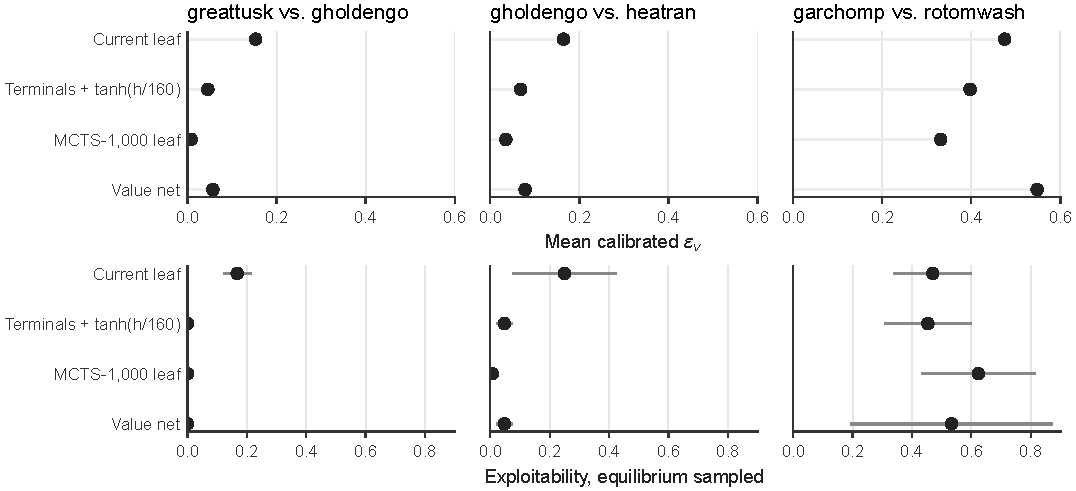
\includegraphics[width=7.18in]{figures/fig_leaves.pdf}
\caption{On the two short endgames every candidate leaf lowers $\epsv$ and exploitability; on garchomp vs.\ rotomwash none lowers exploitability appreciably. Top: mean calibrated $\epsv$ over live states ($n=1{,}162$, $2{,}697$ and $9{,}746$). Bottom: exploitability of equilibrium sampled (payoff units; current-leaf exploitability from the main endgame run; the leaf-comparison harness disagreed on one cell); dot = mean of the two seats, line = seat 1 to seat 2. Values are exact for the abstracted game, so there are no error bars.}
\label{fig:leaves}
\end{figure}

\subsection{RL best response: a negative result}
\label{sec:exp-rl}
We trained PPO best responses on Modal with 100k decisions per target, warm-started from our PPO pilot net on the 12-species full-information pool (not Random Battles), and evaluated each on 200 held-out games.
\begin{table}[h]
\centering\small
\caption{RL best response win rates (95\% CIs about $\pm0.02$--$0.04$ per win rate).}
\label{tab:rl}
\begin{tabular}{@{}lccc@{}}
\toprule
Target & Untrained net & Trained net & Gain \\
\midrule
foul-play, 2,000 it & 0.043 & 0.088 & $+0.045$ \\
Equilibrium, sampled & 0.108 & 0.123 & $+0.015$ \\
Equilibrium, top move & 0.135 & 0.158 & $+0.023$ \\
\bottomrule
\end{tabular}
\vspace{-0.6em}
\end{table}
The best response stays far below 0.5 against every target, so its lower bounds are negative and uninformative. The gains are within noise, except possibly against foul-play ($z\approx2.4$ under independence). The reason is the starting point: the pilot net's final evaluation is 0.0625 against MCTS (intermediate 0--0.135; this ``MCTS-200'' actually ran 1,000 iterations, see Limitations). The RL exploiter used 1.2--2.2k games per target, against the pilot's 340k self-play games. A useful RL exploitability measurement would need a much stronger base policy or a far larger budget. For known targets, white-box search reached a certified lower bound of 0.250 against top move (W1, 100 pairs). Wall time was 0.73\,h, and the budget meter estimated \$2.65 against a \$1.19 plan.

\textbf{RL best response at scale.} To test whether budget was the limit, we reran the best response against foul-play (2,000 iterations) with the same warm start and evaluation (200 held-out games per point, same seeds), planned for 8M decisions (configs \texttt{configs/rlbr\_scale.json} and \texttt{configs/rlbr\_scale\_resume.json}). The run was in two parts: the first stopped at its \$2.92 budget guard after 4.94M decisions, and a resume from that checkpoint (fresh Adam state, constant learning rate $3\times10^{-4}$, new training seeds, 16 games per input) reached 8.01M decisions with no guard stop. The final point is 147k games, about $68\times$ the earlier run's 2.2k games (\cref{tab:rlscale}). The budget meter read \$3.965 in total (\$0.074 smoke, \$2.922 first part, \$0.969 resume) against 13.2 worker core-hours and 2.5\,h wall.
\begin{table}[h]
\centering\small
\caption{RL best response at scale: win rate against foul-play (2,000 iterations) over training, 200 held-out games per point.}
\label{tab:rlscale}
\begin{tabular}{@{}rrcc@{}}
\toprule
Decisions & Games trained & Win rate & 95\% CI \\
\midrule
0 & 0 & 0.060 & [0.036, 0.084] \\
1.00M & 22,016 & 0.065 & [0.042, 0.088] \\
3.01M & 63,232 & 0.090 & [0.064, 0.117] \\
4.94M & 97,536 & 0.100 & [0.071, 0.129] \\
6.00M & 115,200 & 0.1225 & [0.088, 0.157] \\
8.01M & 147,456 & 0.125 & [0.097, 0.153] \\
\bottomrule
\end{tabular}
\vspace{-0.6em}
\end{table}
A $68\times$ increase in training moves the win rate from 0.06 to 0.125, still far below 0.5, so the lower bound on exploitability stays negative (final $-0.375$ [$-0.403$, $-0.347$]). RL gives no useful exploitability bound here, whereas the white-box exploiter certifies $\ge0.250$ (top move) and $\ge0.090$ (sampled) with no training. \emph{Engine detail.} The run was in two parts (see above); the 4.94M checkpoint was evaluated on Modal (0.100) and locally (0.0975) on the same 200 held-out seeds, within sampling noise. The resume cost about \$0.32 per 1M decisions against \$0.59 for the first part, because halving the containers (16 games per input) halved the idle billing.

\subsection{Earlier results, briefly}
\label{sec:exp-earlier}
\textbf{The pruned matrix bug.} poke-engine's iterative-deepening matrix is mostly pruned: 55--80\% of its cells are missing. Treating it as a payoff matrix silently breaks every equilibrium method and invalidated our first round of experiments (E1--E3). With the unpruned full matrix (E1fix), at 2,000 MCTS iterations, equilibrium top move scores 0.581 [0.540, 0.623], safest move 0.561 [0.518, 0.604] and equilibrium sampled 0.443 [0.402, 0.483], at about 25$\times$ MCTS's time per move. Against a fixed opponent, randomizing only costs value, which parallels the lectures' probability-matching example (\cref{sec:prelim}): randomising pays only against an opponent that adapts. RM$^+$ at 100 iterations tied the exact LP in play (0.501 [0.462, 0.541]), but on the pruned matrix, so this is evidence about solvers only.

\textbf{Hidden information (E4, E5).} At equal compute (4 worlds, about 340\,ms per move), agent-form beats the PIMC blend 0.585 [0.540, 0.630] over 400 games. Smaller matchups (100 games) are inconclusive, and the Oracle beats agent-form by about 0.1 (0.600 [0.513, 0.687] sampled play). Over 46,890 logged decisions, blend loss never exceeded the tested $4\delta_H$ bound, where $\delta_H$ is the Hausdorff distance between the worlds' payoff-column sets. The largest loss was 0.098 of the bound, the median loss was 0.19\% of the payoff range, and the top move differed in 14.9\% of decisions. A hand argument tightens the constant to $2\delta_H$; it has been checked by hand only, not formally. Eight worlds did not beat four (X2: 0.495 [0.414, 0.576]), and $\delta_H$ is a weak gate for when to run the joint LP (X3: AUC 0.65), which is also not needed because agent-form costs the same as PIMC.
% CHECK: the 2*delta_H tightening is a hand argument (RESULTS.md "Relation to prior work" item 2); not sent through `prove`. Reported only as such.

\textbf{Experts across battles (X4, X4b, X6).} Offline bootstrap replays with bandit (win/loss) feedback stay inside their regret bounds but need far more battles than a phase of an adaptive opponent lasts. Against the exploiter, Hedge plays the sampled expert 98\% of the time in the last quarter and EXP3 only 56\% (\cref{tab:x4} in \cref{app:tables}). The live learner X6 ($k=3$; top move, sampled, safest), with per-turn counterfactual feedback, matched the best expert against MCTS (0.600 $\pm$ 0.084) and moved to the sampled expert within about 5 battles of meeting an exploiter. X6 used the per-turn normaliser and constant $\eta=0.2$, so only \cref{prop:E1}(a) applies and its regret bound is linear in $S$.

\textbf{Value net and self-play RL.} A value net fit to game outcomes (30k MCTS self-play games, 1.1M positions) predicts no better than the heuristic (held-out sign accuracy 0.743 vs.\ 0.743 for the heuristic on a 2,000-position held-out subsample (0.726 on the full validation set)). As a depth-1 leaf it scores 0.235 [0.185, 0.285] against time-matched MCTS (V1). The roughly 37 positions of a game share one label, so the net mostly learns team strength. Plain PPO self-play (30M decisions, 25 minutes, 12-species full-information pool) reaches a final 0.0625 against MCTS (0--0.135 over training), which was requested at 200 iterations and actually ran 1,000 (see Limitations, \cref{sec:discussion}).
% CHECK: RESULTS.md headline/PPO sections say "MCTS (200 iterations)"; the 2026-11-14 brainstorm section shows poke-engine MCTS always runs >= 1,000 iterations, so every "MCTS-200" was MCTS-1,000. Reported as such.

% =====================================================================
\section{Discussion}
\label{sec:discussion}
\textbf{Strength vs.\ robustness.} No bot dominates. At equal time, foul-play-style MCTS is stronger than equilibrium play (0.650 and 0.760), while equilibrium top move is clearly exploitable by a one-turn LBR (gain 0.183 [0.10, 0.27]) and equilibrium sampling is not detectably so (0.025 [$-0.07$, 0.12]). The depth-2 wb2 exploiter (\cref{tab:wb}) confirms the ordering at 100 pairs: top move 0.873 vs.\ sampled 0.713, difference $+0.160$ [$+0.091$, $+0.229$]. Sampling helps, but it is not robust in absolute terms: wb2 still scores 0.713 and certifies a lower bound of 0.090, consistent with \cref{thm:full}, since stage-wise equilibrium with a bad leaf carries no full-game guarantee. Hedge with carried weights is the one configuration that improves robustness at no detectable cost in strength, and \cref{lem:R3} explains why. The guarantees behind it (\cref{prop:E1}, \cref{thm:E2p}) hold relative to the surrogate, and they transfer to true payoffs only through $\epsv$ (\cref{cor:R4}).

\textbf{The leaf is the bottleneck.} Four independent lines point the same way. (i) The leaf term of \eqref{eq:headline} does not shrink with compute or depth. (ii) Time-matched MCTS wins (X1, E7t). (iii) On exact endgames the calibrated $\epsv$ is near 1 and the bound is loose by 6.9--155$\times$. (iv) A single mis-scored terminal forces $a=0$ (\cref{lem:R6b}), which makes every surrogate-to-true transfer vacuous. Exact terminals fix the easy endgames but not the balanced one.

\textbf{What is preliminary.} The candidate-leaf harness (scratch); the leaf fix's mid-game effect (20 pairs, no measurable change); the X5 hidden-information exploiter (40 games); and the statements R1--R6, which are proved in our notes and checked numerically and were independently verified (2026-11-14), with corrections.

\subsection*{Limitations}
\label{sec:limits}
\begin{itemize}
\item \emph{MCTS batch size.} poke-engine's MCTS runs iterations in batches of 1,000 (the requested count is rounded up), so every ``MCTS-200'' (the PPO pilot's opponent) actually ran 1,000 iterations; the 2,000-iteration settings are exact.
\item \emph{Seeded nondeterminism.} In 1 of 6 local replays the same position produced a different matrix at turn 27, and local and Modal results for the same seed differed. Each game is still a valid sample, but paired-seed pairing is approximate.
\item \emph{White-box pruning.} The 80\% support truncation in W1 affects only the sampled cell, and there is no same-depth non-modelling control, so wb2's score mixes strength and exploitation.
\item \emph{Surrogate units.} Matrices are depth-2 in heuristic engine units, not win probability, and the mapping error is part of $\epsv$, which we cannot measure outside small endgames.
\item \emph{Model simplifications.} Moves count as revealed when chosen, items and abilities are never inferred, the team generator is approximate, and 2--30\% of games hit the 300-turn cap (up to 40\% for LBR in the white-box runs) and count as draws.
\item \emph{Sample sizes.} Most hidden-information matchups have 100 games (CI about $\pm0.09$), the exploitability runs have 30 pairs, and the gains in \cref{tab:lbr} come from different experiments.
\item \emph{Scope.} No Showdown deployment and no ladder result. The behavioural (style) memory, information gathering and concealment from the proposal were not built. Our leaves ignore beliefs, so concealment has zero value in our model (\cref{asm:world}).
\end{itemize}

\textbf{Future work.}
(1) Separating pruning from target play with a $K{=}5$/95\% sampled wb2 cell, plus a same-depth non-modelling control. (2) A value net trained on lower-variance absolute targets (TD bootstrapping, or root values not relative to the root), with exact terminals. (3) Restricted-support deeper leaves, i.e.\ depth-3 lookahead over the equilibrium's support, to attack $\epsv$ where compute allows. (4) Logging $\gamma_{F,t}$ to turn \cref{prop:R3c} into a measured bound. (5) A turn-indexed value or a terminating tie-break near the cap (\cref{prop:R6c}). (6) Showdown deployment through poke-env.

% =====================================================================
\begin{thebibliography}{99}\small
\setlength{\itemsep}{0pt}
% Pokemon
\bibitem{Yu26} M.~Yu. PokaiTrainer: Scaling equilibrium search to competitive Pok\'emon VGC. arXiv:2608.29197 (v2, 28 Sep 2026), 2026.
\bibitem{foulplay} P.~Mariglia. Foul Play: a competitive Pok\'emon Showdown battle bot. \url{https://github.com/pmariglia/foul-play}; engine \url{https://github.com/pmariglia/poke-engine}, 2024.
\bibitem{pokeagent} S.~Karten et~al. The PokeAgent Challenge: competitive and long-context learning at scale. arXiv:2603.15563, 2026.
\bibitem{jaxcalibur} Anonymous (Smogon user jaxcalibur\_author). Jaxcalibur: how Jaxcalibur works. \url{https://jaxcalibur.github.io/} (accessed 2026-11-15); and Smogon thread ``Jaxcalibur: a Gen 9 Randbats bot that reached \#1 on the ladder'', posted 2026-08-28, updated 2026-09-12, \url{https://www.smogon.com/forums/threads/jaxcalibur-a-gen-9-randbats-bot-that-reached-1-on-the-ladder.3787537/} (accessed 2026-11-15). Self-reported, not peer reviewed, code and weights not released.
\bibitem{chrono} TurboRx. Chronoquazicalar. GitHub repository (MIT license), \url{https://github.com/TurboRx/Chronoquazicalar}, 2026; inspected at commit 6e9a7c6, accessed 2026-11-15.
\bibitem{Kar25} S.~Karten, A.~Nguyen, C.~Jin. Pok\'eChamp: an expert-level minimax language agent. arXiv:2503.04094, 2025.
\bibitem{hu2024pokellmon} S.~Hu, T.~Huang, L.~Liu. PokeLLMon: a human-parity agent for Pok\'emon battles with large language models. arXiv:2402.01118, 2024.
\bibitem{grigsby2025metamon} J.~Grigsby et~al. Human-level competitive Pok\'emon via scalable offline reinforcement learning with transformers. arXiv:2504.04395, 2025.
\bibitem{wang2024randbats} J.~Wang. Winning at Pok\'emon Random Battles using reinforcement learning. M.Eng.\ thesis, Massachusetts Institute of Technology, February 2024. \url{https://dspace.mit.edu/handle/1721.1/153888}.
\bibitem{Iha18} H.~Ihara, S.~Imai, S.~Oyama, M.~Kurihara. Implementation and evaluation of information set Monte Carlo tree search for Pok\'emon. IEEE SMC, 2018.
% Game theory, search
\bibitem{Shapley53} L.~S.~Shapley. Stochastic games. Proceedings of the National Academy of Sciences 39(10):1095--1100, 1953.
\bibitem{Kuhn53} H.~W.~Kuhn. Extensive games and the problem of information. In H.~W.~Kuhn and A.~W.~Tucker, eds., Contributions to the Theory of Games II, Annals of Mathematics Studies 28, pp.~193--216. Princeton University Press, 1953.
\bibitem{Sion58} M.~Sion. On general minimax theorems. Pacific J.\ Math.\ 8(1):171--176, 1958.
\bibitem{Fra98} I.~Frank, D.~Basin. Search in games with incomplete information: a case study using Bridge card play. Artificial Intelligence, 1998.
\bibitem{Lon10} J.~Long, N.~R.~Sturtevant, M.~Buro, T.~Furtak. Understanding the success of perfect information Monte Carlo sampling in game tree search. AAAI, 2010.
\bibitem{CFRD} N.~Burch, M.~Johanson, M.~Bowling. Solving imperfect information games using decomposition (CFR-D). AAAI, pp.~602--608, 2014; arXiv:1303.4441.
\bibitem{Mor17} M.~Morav\v{c}\'{\i}k et~al. DeepStack: expert-level artificial intelligence in heads-up no-limit poker. Science, 2017.
\bibitem{Bro17} N.~Brown, T.~Sandholm. Safe and nested subgame solving for imperfect-information games. NeurIPS, 2017.
\bibitem{Bro18} N.~Brown, T.~Sandholm, B.~Amos. Depth-limited solving for imperfect-information games. NeurIPS, 2018.
\bibitem{Bro20} N.~Brown, A.~Bakhtin, A.~Lerer, Q.~Gong. Combining deep reinforcement learning and search for imperfect-information games. NeurIPS, 2020.
\bibitem{Kov23} V.~Kova\v{r}\'{\i}k, D.~Seitz, V.~Lis\'y, J.~Rudolf, S.~Sun, K.~Ha. Value functions for depth-limited solving in zero-sum imperfect-information games. Artificial Intelligence 314:103805, 2023; arXiv:1906.06412.
\bibitem{Tam14} O.~Tammelin. Solving large imperfect information games using CFR+. arXiv:1407.5042, 2014.
\bibitem{Tammelin15} O.~Tammelin, N.~Burch, M.~Johanson, M.~Bowling. Solving heads-up limit Texas hold'em. IJCAI, 2015.
\bibitem{BMS19} N.~Burch, M.~Morav\v{c}\'{\i}k, M.~Schmid. Revisiting CFR+ and alternating updates. JAIR 64:429--443, 2019; arXiv:1810.11542.
\bibitem{BLM13} S.~Boucheron, G.~Lugosi, P.~Massart. Concentration Inequalities: A Nonasymptotic Theory of Independence. Oxford University Press, 2013.
\bibitem{Hannan57} J.~Hannan. Approximation to Bayes risk in repeated play. In M.~Dresher, A.~W.~Tucker, P.~Wolfe, eds., Contributions to the Theory of Games III, Annals of Mathematics Studies 39, pp.~97--139. Princeton University Press, 1957.
\bibitem{LW94} N.~Littlestone, M.~K.~Warmuth. The weighted majority algorithm. Information and Computation 108(2):212--261, 1994.
\bibitem{CS535L6} CS535 Algorithmic Game Theory, Lecture 6: Learning in Games and Playing Against Nature; Lecture 7: No-Regret Dynamics in Games, 2026.
\bibitem{FS97} Y.~Freund, R.~E.~Schapire. A decision-theoretic generalization of on-line learning and an application to boosting. J.\ Computer and System Sciences 55(1):119--139, 1997.
\bibitem{HW98} M.~Herbster, M.~K.~Warmuth. Tracking the best expert. Machine Learning 32(2):151--178, 1998.
\bibitem{CBL06} N.~Cesa-Bianchi, G.~Lugosi. Prediction, Learning, and Games. Cambridge University Press, 2006.
\bibitem{Aro12b} R.~Arora, O.~Dekel, A.~Tewari. Online bandit learning against an adaptive adversary: from regret to policy regret. ICML, 2012.
\bibitem{OP18} F.~Orabona, D.~P\'al. Scale-free online learning. Theoretical Computer Science 716:50--69, 2018; arXiv:1601.01974.
\bibitem{Gan15} S.~Ganzfried, T.~Sandholm. Safe opponent exploitation. ACM Trans.\ Economics and Computation, 2015.
\bibitem{Joh09} M.~Johanson, M.~Bowling. Data biased robust counter strategies. AISTATS, 2009.
\bibitem{Saf12} A.~Saffidine, H.~Finnsson, M.~Buro. Alpha-beta pruning for games with simultaneous moves. AAAI, 2012.
\bibitem{Bos16} B.~Bo\v{s}ansk\'y, V.~Lis\'y, M.~Lanctot, J.~\v{C}erm\'ak, M.~H.~M.~Winands. Algorithms for computing strategies in two-player simultaneous move games. Artificial Intelligence, 2016.
\bibitem{Lis13} V.~Lis\'y, V.~Kova\v{r}\'{\i}k, M.~Lanctot, B.~Bo\v{s}ansk\'y. Convergence of Monte Carlo tree search in simultaneous move games. NeurIPS, 2013.
\bibitem{Tim20} F.~Timbers et~al. Approximate exploitability: learning a best response in large games. arXiv:2004.09677, 2020.
\bibitem{Everett57} H.~Everett. Recursive games. In Contributions to the Theory of Games III, Annals of Mathematics Studies 39. Princeton University Press, 1957.
\bibitem{DS65} L.~E.~Dubins, L.~J.~Savage. How to Gamble If You Must: Inequalities for Stochastic Processes. McGraw-Hill, New York, 1965 (2nd ed., Dover, 1976).
\bibitem{MS96} A.~P.~Maitra, W.~D.~Sudderth. Discrete Gambling and Stochastic Games. Springer, New York, 1996; doi:10.1007/978-1-4612-4002-0. % CHECK CITE: theorem numbers and the ``conserving'' terminology unchecked (book not read).
\bibitem{KL02} S.~Kakade, J.~Langford. Approximately optimal approximate reinforcement learning. ICML, 2002.
\bibitem{Wei21} C.-Y.~Wei, C.-W.~Lee, M.~Zhang, H.~Luo. Last-iterate convergence of decentralized optimistic gradient descent/ascent in infinite-horizon competitive Markov games. COLT, 2021. % CHECK VENUE
\bibitem{DFG20} C.~Daskalakis, D.~J.~Foster, N.~Golowich. Independent policy gradient methods for competitive reinforcement learning. NeurIPS, 2020. % CHECK VENUE
\bibitem{EKM09} E.~Even-Dar, S.~M.~Kakade, Y.~Mansour. Online Markov decision processes. Mathematics of Operations Research 34(3):726--736, 2009.
\bibitem{Aga21} A.~Agarwal, S.~M.~Kakade, J.~D.~Lee, G.~Mahajan. On the theory of policy gradient methods: optimality, approximation, and distribution shift. JMLR 22(98), 2021.
\bibitem{Whi91} S.~D.~Whitehead. A complexity analysis of cooperative mechanisms in reinforcement learning. AAAI, 1991. % CHECK VENUE
\bibitem{Kak03} S.~M.~Kakade. On the sample complexity of reinforcement learning. PhD thesis, University College London, 2003. % CHECK VENUE
\bibitem{KL19} V.~Kova\v{r}\'{\i}k, V.~Lis\'y. Analysis of Hannan consistent selection for Monte Carlo tree search in simultaneous move games. Machine Learning, 2019.
\bibitem{Per16} J.~P\'erolat, B.~Piot, B.~Scherrer, O.~Pietquin. Softened approximate policy iteration for Markov games. ICML, 2016. % CHECK VENUE
\end{thebibliography}

% =====================================================================
\appendix
\section{Proof sketches}
\label{app:proofs}
Full proofs are in \texttt{theory/full\_game.md}, \texttt{theory/hedge\_experts.md} and \texttt{theory/regret\_theory.md}.

\textbf{\Cref{thm:full}.} Fix $\sigma$. Define $D_t(h)=\delta(t,s_t)+\E[D_{t+1}\mid h]$ on live histories and $0$ otherwise. If $W_{t+1}\ge\Vstar_{t+1}-D_{t+1}$ on every child, then $W_t(h)\ge x^\top\Qstar_t(s)y-(D_t-\delta)$ with $y=\sigma(h)$. \Cref{lem:one} gives $x^\top\Qstar_ty\ge\Vstar_t(s)-\delta$, which closes the induction. The opponent's conditioning on past realised actions is harmless because the induction runs over histories. Taking the infimum over $\sigma$ and choosing $\sigma=\sigma^\star$ gives \eqref{eq:full}.

\textbf{\Cref{prop:rm} for the code's indexing.} Add one virtual row update. Then $W[u(a,\bar y)-u(\bar x,\beta)]=\sum_tt\,r^x_{t+1}(a)+\sum_tt\,r^y_t(\beta)+\sum_tt\,[u(x_t,y_t)-u(x_t,y_{t-1})]$. The last sum is $\le0$ term by term (\cite{BMS19}, Thm~5), and the weighted regret bound gives $\mathrm{gap}\le2\Delta(\sqrt{n(T+1)}+\sqrt{mT})/(T+1)$. The uniform-fallback case ($Q=0$) was checked by reading.

\textbf{\Cref{thm:C}.} Because the samples are fresh and unobserved, the opponent faces the expected mixture $\tilde x$. The agent-form objective $f_b$ is concave, so $f_b(\tilde x)\ge v(b)-(\epss+2\epsv+2\E S)$. Two applications of $|f_b-f_p|\le\Delta\TV(b,p)$ convert this to the true posterior $p$. The revealed stage payoff and the true belief-dependent payoff $\Phi_p$ differ by at most $\etaNL$, and $V_t(s,p)\le\max_x\min_y\Phi_p$ (convexity of $V_t$ in the belief, perspective functions, Sion's theorem~\cite{Sion58}). The induction then mirrors \cref{thm:full}.

\textbf{\Cref{prop:R1}.} Write $s_n=\sum_{j\le n}j^{-1/2}$, so $2\sqrt{n+1}-2\le s_n\le2\sqrt n$. After phase 1, $\Lambda_t=\lambda_t(1)-\lambda_t(2)=c(2s_{T_1}-s_{t-1})$. For $t\le4\theta^2T_1$ this gap is $\ge2c(2(1-\theta)\sqrt{T_1}-2)\to\infty$, so the learner misses phase-2 reward until $4\alpha T$. For $t\ge4T_1/\theta^2$ it goes to $-\infty$. Letting $\theta\uparrow1$ gives matching $\liminf$ and $\limsup$.

\textbf{\Cref{prop:R5b}.} The identity follows by adding and subtracting $s(\pi,\beta)$. The bound follows from $s(\pi,X)\ge v^\star-\expl(\pi)$ and $s(\pi,\beta)\le v^\star+\expl(\beta)$ in a symmetric game with value $1/2$.

\textbf{\Cref{lem:R6b}.} For fixed $a$, the best $c$ centres $aM_i-Q_i$, giving $\frac12\max_{i,j}[(Q_i-Q_j)-a(M_i-M_j)]$. This is convex and piecewise linear in $a$, and $a=0$ is optimal iff its right derivative at $0$ is $\ge0$, i.e.\ iff some active pair $(i\in\argmax Q,\ j\in\argmin Q)$ has $M_i\le M_j$.

\section{Verification status}
\label{app:status}
\begin{table}[h]
\centering\small
\caption{How each statement was checked. ``Lean'' $=$ Lean~4/Mathlib, no \texttt{sorry}, axioms only propext / Classical.choice / Quot.sound (\texttt{theory/lean/FullGame/\{Basic,Hedge\}.lean}). ``Reading'' $=$ adversarial line-by-line check (\texttt{theory/CHECK.md}). ``Numeric'' $=$ scripts in \texttt{theory/checks/}.}
\label{tab:status}
\begin{tabular}{@{}p{0.36\linewidth}p{0.6\linewidth}@{}}
\toprule
Statement & Status \\
\midrule
\Cref{lem:one}, factor 2 tight & Lean (\texttt{lemma1\_one\_step}, \texttt{lemma1\_mixed}; tightness \texttt{example}) \\
$|\val A-\val B|\le\lVert A-B\rVert_\infty$ & Lean (\texttt{val\_lipschitz}, \texttt{exists\_val}) \\
\Cref{thm:full} induction & Lean in abstract form (\texttt{backward\_induction}, \texttt{deficit\_le\_sum}, \texttt{theoremA\_abstract}); game-model link by reading \\
$\Hbar$ refinement and counterexample (\cref{rem:hbar}) & Reading and brute force \\
\Cref{prop:rm} for the code's RM$^+$ & Key step in Lean (\texttt{rmplus\_improvement} $=$ \cite{BMS19} Thm~5); constant by reading; numeric ratio 0.12--0.20 \\
\Cref{prop:K} & Reading and simulation; vacuous at small $K$ \\
\Cref{thm:C}, three-type example & Reading; example brute-forced (\texttt{example\_c1\_repaired.py}) \\
$\sum_t(\etaNL+4\TV)\approx$ oracle gap & Conjecture \\
\Cref{lem:H} (Hedge, fixed share) & Summation step in Lean (\texttt{hedge\_telescope}); per-step Hoeffding is a hypothesis, checked by reading \\
\Cref{prop:E1}(a),(b) & Lean (\texttt{claim1\_weighted}, \texttt{claim1\_fixed}, \texttt{learner\_reward\_linear}); raw-unit (a) false, counterexample brute-forced \\
Theorem E2 (constant $\eta$) & Per-turn step in Lean (\texttt{composition\_step}); telescoping by reading; checked by an independent verifier for constant $\eta$ \\
E3 and its policy-regret caveat & Reading; cited~\cite{Aro12b} \\
R1--R6 (\cref{lem:R2,thm:E2p,prop:R1,lem:R3,prop:R3c,cor:R4,prop:R5a,prop:R5b,prop:R5c,lem:R6a,lem:R6b,prop:R6c}) & Proved in \texttt{regret\_theory.md}, checked numerically (\texttt{rt1}--\texttt{rt6}); independently verified (2026-11-14), with corrections (numeric brute force + proof reading). R4 reuses the Lean \texttt{composition\_step} \\
Cited, not re-proved & Shapley~\cite{Shapley53}; Kuhn~\cite{Kuhn53}; Sion~\cite{Sion58}; Hoeffding and the sub-Gaussian maximal inequality~\cite{BLM13}; \cite{BMS19} Thm~8; \cite{CBL06} Thm~2.3; Everett, Dubins--Savage; DeepStack/ReBeL/CFR-D bounds (not used in proofs) \\
\bottomrule
\end{tabular}
\end{table}

\section{Additional tables}
\label{app:tables}
\begin{table}[h]
\centering\small
\caption{X4/X4b: EXP3 and Hedge over whole-battle experts, offline bootstrap replay (mean score per battle; regret vs.\ the best fixed expert in battles in parentheses). X4: 2,000 repeats; X4b: 1,000 repeats.}
\label{tab:x4}
\begin{tabular}{@{}lccccc@{}}
\toprule
Scenario & Best fixed & EXP3 & Hedge & Fixed-share Hedge & Uniform \\
\midrule
vs.\ MCTS-2000, $N=400$ & 0.581 & 0.541 (16.0) & 0.566 (6.2) & -- & 0.528 (21.2) \\
vs.\ MCTS-2000, $N=4{,}000$ & 0.581 & 0.557 (95.4) & 0.575 (26.7) & -- & 0.528 (212.2) \\
exploiter only, $N=400$ & 0.475 & 0.406 & 0.454 & 0.444 & 0.386 \\
MCTS-2000 300, then exploiter 300 & 0.464 & 0.457 & 0.460 & 0.478 & 0.458 \\
\bottomrule
\end{tabular}
\end{table}

\begin{table}[h]
\centering\small
\caption{X6 live learner ($k=3$, Hedge $\eta=0.2$ + fixed share $\alpha=0.002$, per-turn normaliser), 3 seeds $\times$ 80 battles. $\pm$ is the 95\% CI half-width $1.96\,\mathrm{sd}/\sqrt n$ over the $n=120$ battles pooled across seeds.}
\label{tab:x6}
\begin{tabular}{@{}lcl@{}}
\toprule
Phase & Learner score & Fixed experts in the same setting \\
\midrule
vs.\ MCTS-2000, battles 0--39 & 0.600 $\pm$ 0.084 & top move 0.58, safest 0.56, sampled 0.44 \\
vs.\ exploiter, battles 40--49 & 0.417 & vs.\ own exploiter: sampled 0.475, safest 0.367, top move 0.317 \\
vs.\ exploiter, battles 50--59 & 0.400 & \\
vs.\ exploiter, battles 60--79 & 0.458 & \\
\bottomrule
\end{tabular}
\end{table}

\begin{table}[h]
\centering\small
\caption{R3b: logged vs.\ predicted MCTS-expert weight $w_F$ (carried weights, mean over 4 seeds; constant-slope model of \cref{lem:R3}(b) with pooled $d_1,d_2$).}
\label{tab:r3b}
\begin{tabular}{@{}lccccccc@{}}
\toprule
Game & 0 & 9 & 19 & 29 & 39 & 49 & 59 \\
\midrule
Mean learner turns $t$ & 45 & 332 & 640 & 1028 & 1462 & 1934 & 2505 \\
Logged $w_F$ & 0.452 & 0.359 & 0.306 & 0.278 & 0.162 & 0.106 & 0.072 \\
Predicted $w_F$ & 0.450 & 0.362 & 0.312 & 0.268 & 0.166 & 0.106 & 0.065 \\
\bottomrule
\end{tabular}
\end{table}

\end{document}
